\documentclass[
	12pt,
	a4paper,
	BCOR10mm,
	%chapterprefix,
	DIV14,
	listof=totoc,
	bibliography=totoc,
	headsepline
]{scrreprt}

\usepackage[T1]{fontenc}
\usepackage[utf8]{inputenc}
\usepackage{wrapfig}

%\usepackage[ngerman, USenglish]{babel}
\usepackage[ngerman]{babel}
\usepackage{lmodern}

\usepackage[footnote]{acronym}
\usepackage[page,toc]{appendix}
\usepackage{fancyhdr}
\usepackage{float}
\usepackage{graphicx}
\usepackage[pdfborder={0 0 0}]{hyperref}
\usepackage[htt]{hyphenat}
\usepackage{listings}
\usepackage{lscape}
\usepackage{microtype}
\usepackage{nicefrac}
%\usepackage{subfig}
\usepackage{textcomp}
\usepackage[subfigure,titles]{tocloft}
\usepackage{units}
\usepackage{graphicx}
\usepackage{caption}
\usepackage{subcaption}



\lstset{
	basicstyle=\ttfamily,
	frame=single,
	numbers=left,
	language=python,
	breaklines=true,
	breakatwhitespace=true,
	postbreak=\hbox{$\hookrightarrow$ },
	showstringspaces=false,
	tabsize=4
}

\renewcommand*{\lstlistlistingname}{Listingverzeichnis}

\renewcommand*{\appendixname}{Anhang}
\renewcommand*{\appendixtocname}{Anhänge}
\renewcommand*{\appendixpagename}{Anhänge}


\setcounter{tocdepth}{1} 

\begin{document}

\begin{titlepage}
	\begin{center}
		{\titlefont\huge Implementierung von Skelettierungs-Algorithmen mit dem Kinect-Sensor\par}

		\bigskip
		\bigskip

		{\titlefont\Large --- Projektbericht ---\par}

		\bigskip
		\bigskip

		{\large Arbeitsbereich Kognitive Systeme\\
		Fachbereich Informatik\\
		Fakultät für Mathematik, Informatik und Naturwissenschaften\\
		Universität Hamburg\par}
	\end{center}
	
	\vfill
	
	{\large \begin{tabular}{ll}
		Vorgelegt von: & Johannes Böhler, \\
				& Christopher Kroll, \\ 
				& Sandra Schröder (6060939) \\\\
		Hamburg, den 10.03.2013
	  \end{tabular}\par}

\end{titlepage}

\newcommand{\Autor}[1]{{\hfill \Large \textit{Autor: #1}}}

\chapter*{Zusammenfassung}

\thispagestyle{empty}

Abstract über unseren Projektbericht

\tableofcontents
\chapter{Einleitung}
\Autor{Christopher Kroll}\\ \\
Im Master-Studiengang Informatik an der Universit"at Hamburg ist ein zweisemestriges Projekt vorgesehen. Die Autoren dieser Arbeit belegten im Sommersemester 2012 und Wintersemester 2012/2013 das Projekt 'Bildverarbeitung' unter der Leitung von Prof. Dr. Leonie Dreschler-Fischer. 
%TODO: Die anderen beiden auch aufz�hlen?
Der Verlauf und das Ergebnis dieses Projektes wird in dem vorliegenden Dokument dargestellt.
\\ \\
Die Studenten sollten in diesem Projekt die Daten der Microsoft Kinect-Kamera nutzen und diese f"ur ein Thema ihrer Wahl verarbeiten. Nach einer Vorstellung der Kinect und der Programmiersprache Python wurden die Gruppen eingeteilt und das Thema gew"ahlt (siehe Kapitel \ref{aufgabenstellung} ).  \\ 

Die digitale Bildverarbeitung hilft unter anderem bei der Erkennung von Objekten, wie zum Beispiel bei der vollautomatisierten Qualit"atskontrolle. Um auch bei gro"sen Datenmengen noch performant arbeiten zu k"onnen, bedient man sich oft des Mittels der Abstraktion. Das Projektthema dieser Arbeit dreht sich um eine M"oglichkeit der Abstraktion, n"amlich der Skelettierung. \\
Der Begriff 'Skelett' taucht in vielen Fachbereichen, wie zum Beispiel der Anatomie, Biologie oder Architektur auf. In der digitalen Bildverarbeitung hat er einen "ahnlichen Sinn wie in diesen Bereichen: Es stellt von einem Objekt das Grundger"ust dar. Dieses Ger"ust ist der zentrale Hauptbestandteil, mit dessen Hilfe sich R"uckschl"usse auf das gesamte Objekt (siehe Dinosaurierskelette) ergeben. \\
Aus Sicht der Bildverarbeitung kann ein Skelett folgenderma"sen definiert werden: Ein Skelett ist ein n"utzlicher Deskriptor, um Informationen "uber die Region und den Rand eines Objektes kompakt und effizient zu kodieren und gibt die wesentlichen Grundz"uge eines Objektes wieder. In diesem Fachbereich kommen noch weitere Eigenschaften des Skeletts hinzu. Das Ziel ist die Information eines Objektes zu reduzieren ohne dabei die Grundstruktur zu verletzen. So ist eine Anforderung, dass die 'Pixelkonnektivit"at' gew"ahrleistet ist, also alle sp"ateren Skelettpixel mindestens einen benachbarten Skelettpixel besitzen und das Skelett nicht unterbrochen ist. \\
Bei der Skelettierung muss weiterhin beachtet werden, dass die topologische Struktur des Originalbildes nicht ver"andert wird. Trotz eventueller Verformung bei der Skelettbildung, wie in Abbildung \ref{fig:topologischeStruktur} dargestellt, muss die strukturelle Eigenschaft erhalten bleiben; so ist bei einer automatisierten Zeichenerkennung die Strichst"arke unerheblich, lediglich der generelle Aufbau des Buchstaben ist relevant. \\
%
\includegraphics[width=1.0\linewidth]{./fig/topologischeStruktur}
\begin{figure}
\centering

\includegraphics[width=0.7\linewidth]{./fig/topologischeStruktur}
\caption{Skelettierung des Buchstaben A TODO cite \cite{TODO cite?}}
\label{fig:topologischeStruktur}
\end{figure}

TODO  geschichte und 3 Gruppen der skelettierung


\section{Aufgabenstellung}
\label{aufgabenstellung}
Unsere Gruppe entschied sich f"ur die Datenauswertung einer Person ('Spieler'). Dabei war zun"achst das Ziel den Bewegungsablauf bei Sport"ubungen zu analysieren und eine R"uckmeldung zu geben, ob diese richtig ausgef"uhrt wurden. So soll zum Beispiel bei Kniebeugen durch eine Messung des Winkels zwischen Ober- und Unterschenkel der Person eine Hilfestellung gegeben werden. \\ \\ 
Um dieses Ziel zu erreichen muss zun"achst der Spieler von anderen Gegenst"anden im Raum getrennt, also herausgefiltert werden (Segmentierung). F"ur die Bewegungsanalyse ist es hilfreich nicht den gesamten Menschen, wom"oglich noch mit st"orender Kleidung, zu betrachten, sondern nur sein Skelett. Um das Skelett zu erhalten, bot sich die Wahl zwischen schon implementierten Skelettierungsalgorithmen zu benutzen oder dies selbst zu implementieren. Da das Thema des Projektes die Bildverarbeitung und nicht eine Anwendungsprogrammierung ist, fiel die Entscheidung auf die Konzentration auf die Skelettierung. Das Ziel war nun verschiedene Ans"atze zu implementieren und hinsichtlich Qualit"at und Leistung zu vergleichen.  \\ \\
Dabei mussten einige Kriterien beachtet werden. Zuallererst muss auf die Qualit"at des erzeugten Skeletts geachtet werden. Es sollte als eine Skelettrepr"asentation des Quellbildes erkannt werden, also ein zentrales Grundger"ust mit vorhandener Pixelkonnektivit"at. Desweiteren ist die Leistungsf"ahigkeit relevant. Die Algorithmen sollen echtzeitf"ahig sein, damit der Spieler eine unmittelbare R"uckmeldung seiner Bewegungen erh"alt.
\section{Aufbau der Projektarbeit}
TODO am ende wenn struktur steht
\chapter{Aufgabenstellung}


\section{Anforderungen}
\section{Die Kinect}
Die drei Haupt Hardware-Komponenten der Kinect sind ein Infrarot Projektor, eine Infrarot Kamera sowie eine Infrarot Kamera.

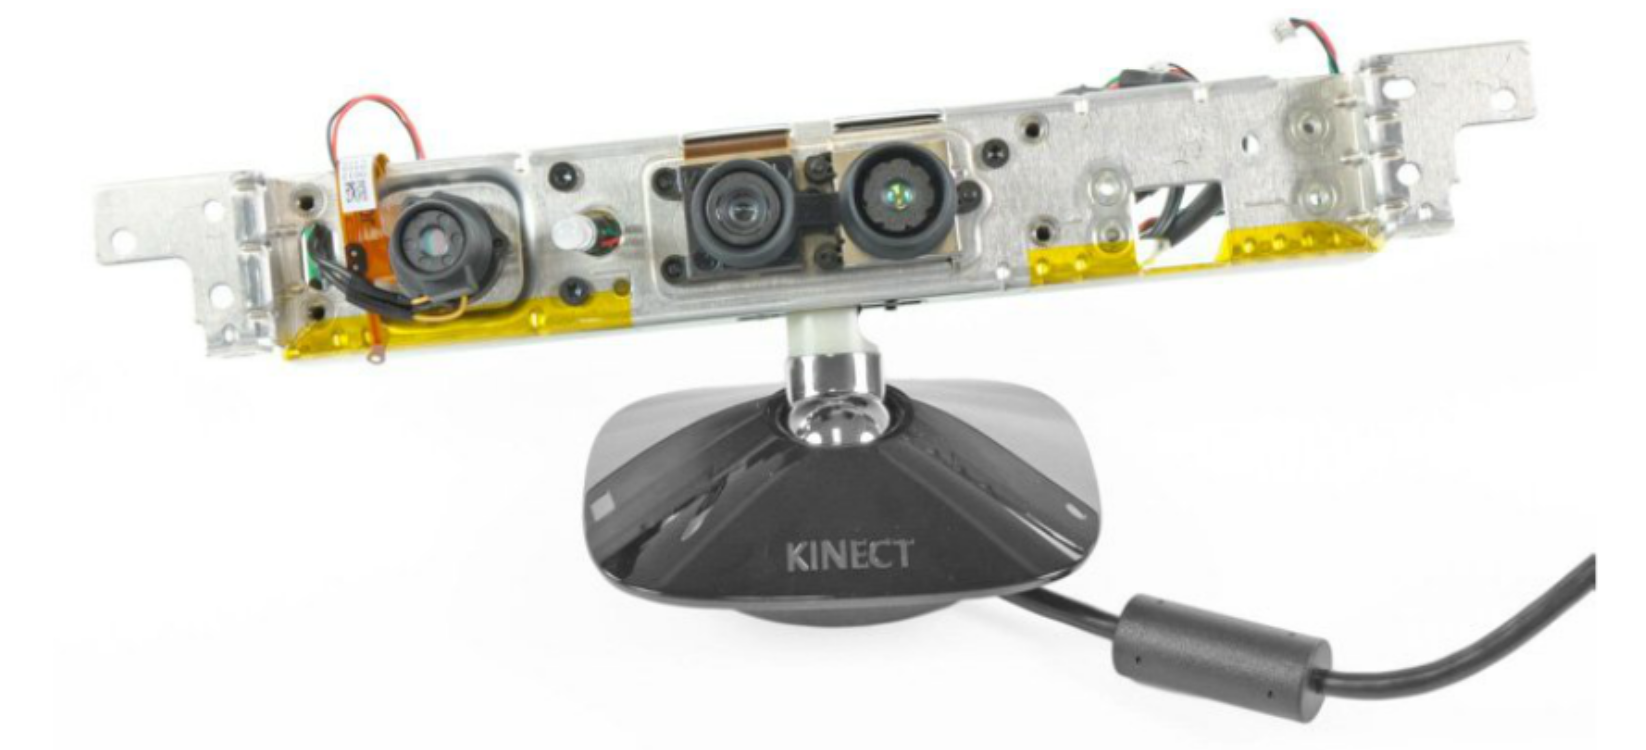
\includegraphics[height=5cm]{Res/Kinect_Components.png}



Die Kombination aus Infrarot Strahler und Infrarot Kamera ermöglicht die Gewinnung von Tiefeninformationen aus der Umgebung. Im Gegensatz zu gewöhnlichen Kameras welche einem Pixel Farbinformation (z.B.  über RGB-Farbkanäle) zuordnen, wird dem Pixel mit Hilfe der Infrarot Kamera eine Entfernung zugeordnet. Diese ergibt sich aus der Art und Weise wie der Infrarotstrahl von dem durch den Pixel repräsentierten Bereich eines Objektes reflektiert wurde.

Die Tiefenbilder welche man von der IR Kamera erhält, sehen aus wie komplett verrauschte Graustufenbilder. Hierbei steht jeder Grau Wert eines Pixels für die entsprechende Entfernung des korrespondierenden Objektausschnittes zur Kinect.



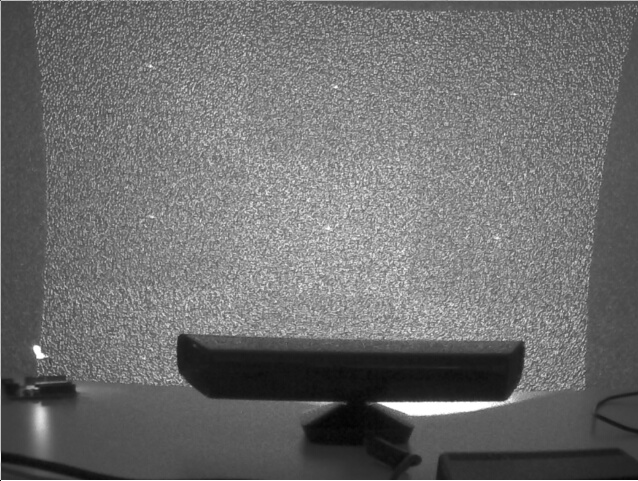
\includegraphics[height=5cm]{Res/Kinect_9Points.png}



Hohe Grauwerte (helle Pixel) repräsentieren nahe Objekte während niedrige Grauwerte (dunkle Pixel) weiter entfernte Objekte beschreiben. In einem Tiefenbild ist die gesamte Information über die Entfernung der im Bildausschnitt erfassten Objekte zur Kinect enthalten.

Wird die Tiefeninformation dazu genutzt um die Pixel mit Hilfe der durch die RGB Kamera erfassten Farbwerte der XY Koordinaten im dreidimensionalen Raum anzuordnen, erhält man eine sogenannte (farbige) Punktwolke. Die in der 2d 
-Betrachtung benachbarte Pixel müssen in der 3d Repräsentation nicht miteinander verbunden da die Z-Koordinate unterschiedliche Werte aufweisen kann.
\subsection{Funktionale Komponenten}
\subsubsection{Infrarotprojektor}

Der Infrarotprojektor emittiert elektromagnetische Strahlen, deren Wellenlänge (830nm) außerhalb des für den Menschen sichtbaren Bereichs liegt (380nm-780nm).
Der Projektor strahlt zur Tiefenbestimmung ein Gitter von Infrarotpunkten (strukturiertes Licht) auf die Objekte in seiner Umgebung ab. 
Die Firma PrimeSense (welche von Microsoft aufgekauft wurde) implementiert ein besonderes Verfahren zur Generierung dieses Musters.
Normalerweise produzieren Filter die diese Art von Muster generieren einen sehr hellen Punkt in der Mitte des Bildes, welcher die Leistungsfähigkeit des IR Projektors limitiert.\\


Durch das hier angewandte Verfahren entstehen statt einem einzigen sehr hellen, neun helle Punkte, welche durch unvollständige Lichtfilterung zur Mustererstellung bedingt sind. Das hier eingesetzte Verfahren produziert weniger starke Artefakte und ermöglicht die Verwendung einer leistungsfähigeren Diode was eine erhöhte Genauigkeit sowie eine größere Reichweite ermöglicht. . Trotzdem ist die Reichweite des IR Projektors eingeschränkt, da zu hohe Intensitäten der IR Strahlen Augenschäden verursachen könnten.


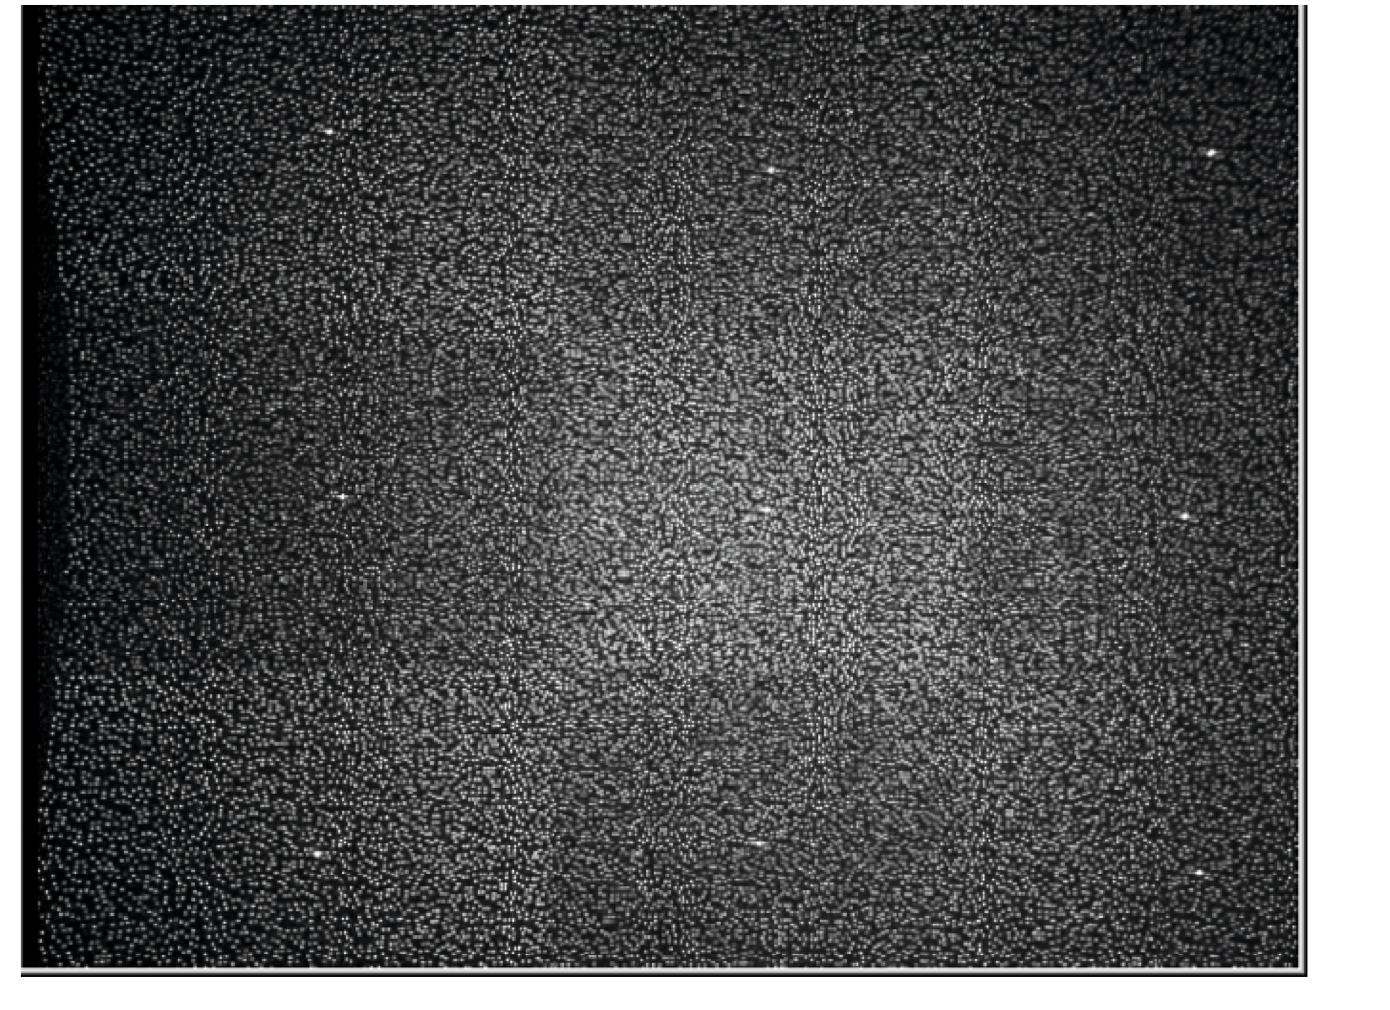
\includegraphics[height=5cm]{Res/9_Dots.png}



Es ist wichtig dass die Wellenlänge der Infrarot strahlen konstant bleibt, was durch eine konstante Temperatur der Laserdiode und eine konstante Stromleistung (60 mW) gewährleistet wird. Problem hierbei sind variierende Außentemperaturen(die empfohlene Betriebstemperatur  liegt zwischen 5 und 35 °C). Um diese Konstanz zu gewährleisten wird ein sogenanntes  Peltier-Element verwendet, welches sowohl kühlen als auch wärmen kann.\\

\subsubsection{Infrarotkamera}


Die IR Kamera nimmt Bilder mit einer nativen Auflösung von 1280x1024 Pixeln bei einer Bildwiederholrate von 30 Hz auf. Weitergeleitet werden allerdings nur Bilder mit einer Auflösung von 640x480 Pixeln da der USB Datenbus eine Limitierung bezüglich übertragbarer Datenraten darstellt. Das Blickfeld der IR Kamera beträgt in der Horizontalen 58 °, in der Vertikalen 45 °. Damit sich die Mustererkennung funktioniert ist eine Mindestabstand von 0,8 Metern erforderlich, ab einer Entfernung von 3,5 Metern wird die Intensität der reflektierten Strahlen zu gering um Tiefeninformationen mit ausreichender Präzision zu erhalten.\\

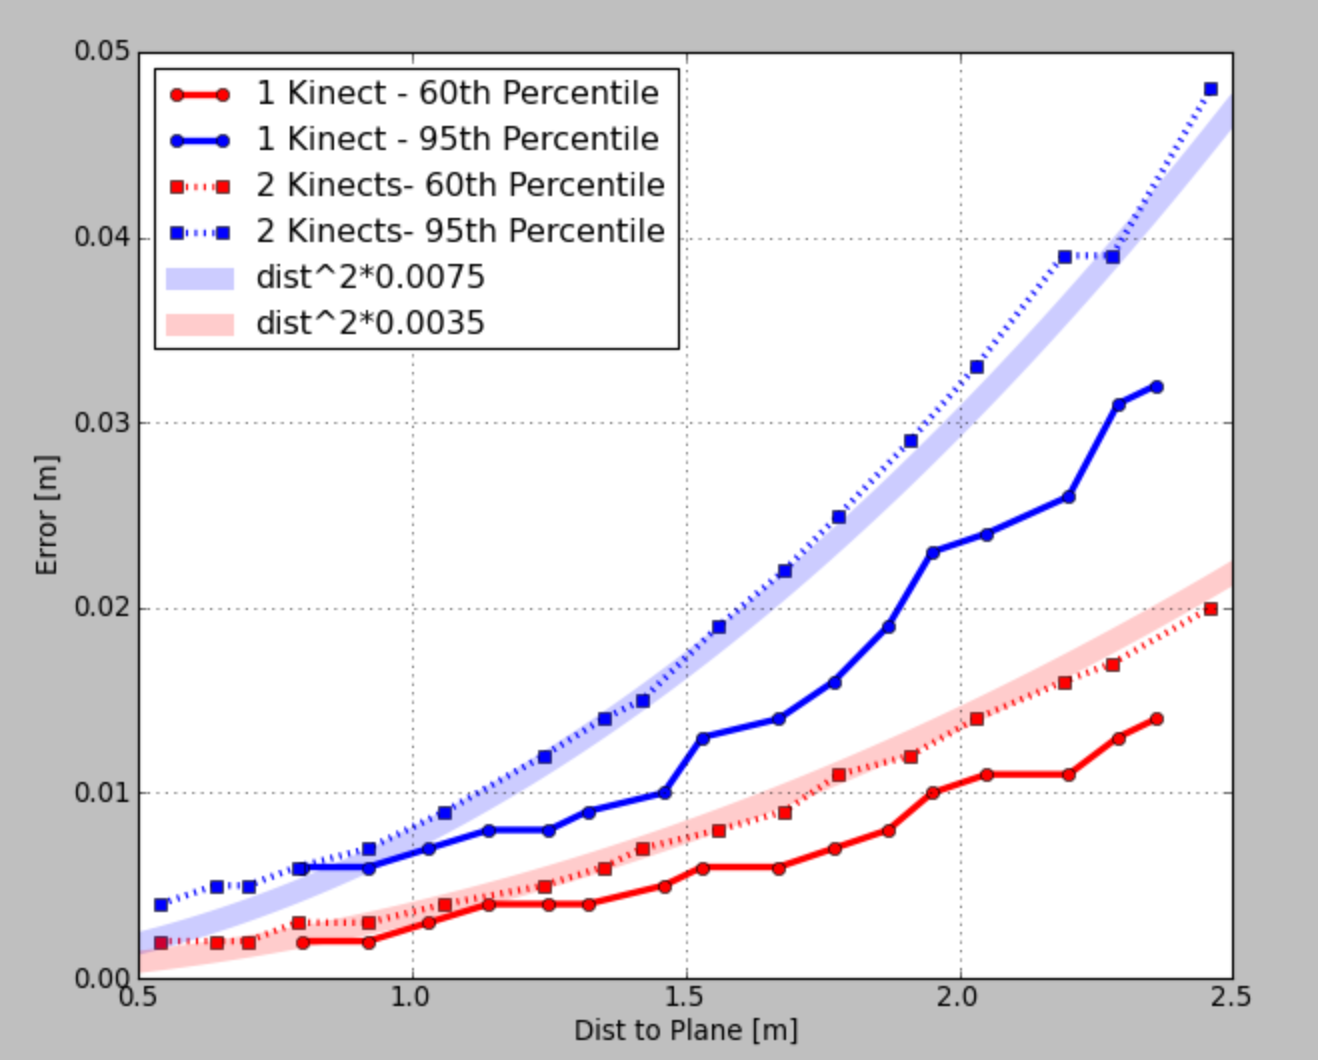
\includegraphics[height=5cm]{Res/Res_to_Dist.png}

Bei einem optimalen Abstand von 2 Metern zum Objekt beträgt die Auflösung in der XY Ebene 3mm, in der Z Ebene 1cm.
Die Quantisierungsauflösung liegt bei  (2048) Bit.
Es muss sichergestellt werden dass die IR Kamera nur die erwünschte elektromagnetische Strahlung im 830 nm Bereich aufnimmt und nicht von Strahlungen anderer Wellenlänge gestört wird . Die wird durch einen Filter welcher auf dem IR Kameraobjektiv angebracht ist realisiert.
Trotz des Filters sollte die Kinect eher in abgedunkelten Innenräumen verwendet werden, da im Sonnenlicht auch elektromagnetische Wellen im Infrarotbereich enthalten sind.\\

\subsubsection{RGB Kamera}

Die RGB Kamera nimmt bei einer Wiederholrate von 30 Hz ebenfalls mit einer Auflösung von 640x480 Pixeln auf, könnte aber alternativ auch mit einer Auflösung von 1280x1024 Pixeln bei einer reduzierten Wiederholrate von 15 Bildern pro Sekunde angesteuert werden.
Die Quantisierungsauflösung liegt hier bei  (256)Bit. \\


\subsubsection{Mikrofon Array}
Die Kinect beinhaltet vier Mikrofone welche verteilt verbaut sind. Sie dienen sowohl der Erfassung von Ton, als auch der Lokalisierung und Unterscheidung von Soundquellen. Jedes der Mikrophone tastet mit einer Quantisierungsauflösung von  (65536) Bit und einer Abtastrate von 16 KHz ab.

\subsection{Tiefenberechnung}

Die Berechnung der Objektentfernungen (Tiefenwerte) innerhalb der Kinect erfolgt durch Aussendung von strukturiertem Licht durch die Projektionseinheit und durch Weiterverwertung  der durch die IR empfangen reflektierten Strahlen auf einem Chip der Firma PrimeSense (PS1080-A2-Chip). Das Muster für das strukturierte Licht wird mit Hilfe eines Diffusors(einer Lochplatte mit fest definiertem Muster) erzeugt.\\
Das Prinzip des Strukturierten Lichts ist an ein Verfahren angelehnt, welches sich Streifenprojektion nennt und in dieser Anwendung abgewandelt wurde um die Erfassung von beweglichen Objekten zu ermöglichen. Statt Lichtstreifen wird bei dem von der Kinect angewendeten Verfahren eine Punktematrix verwendet, welche fest definiert ist. Die IR Kamera sowie der Projektor müssen sich hierzu in einem fest definiertem, gleich großem Abstand zueinander befinden.
Die Umgebungsreflektionen der projizierten Punktematrix werden von der Infrarotkamera erfasst.
Um aus diesem Gitter von Infrarotpunkten Tiefeninformation extrahieren zu können wird das Verfahren der aktiven Stereotriangulation verwendet.\\


Die Triangulation ist ein Verfahren zur optischen Abstandsmessung welches sich hierzu trigonometrischer Funktionen innerhalb von aufgespannten Dreiecken bedient. 
Es wird allgemein zwischen aktiver und passiver Triangulation unterschieden.
Aktive Triangulation bedeutet dass mindestens eine strukturierte Lichtquelle zur Abstandsberechnung erforderlich ist, während dies bei passiver Triangulation nicht der Fall ist.
Da der IR Projektor ein statisches Pseudozufallsmuster emittiert, ist dieser als strukturierte Lichtquelle einzuordnen.
Stereotriangulation bedeutet dass zwei unterschiedliche Bildquellen benötigt werden um die Tiefe jedes Pixels eines Bildausschnittes berechnen zu können.
Eine Bildquelle ist der Diffusor (das „Lochmuster“) welcher die vom Projektor emittierten Strahlen statisch definiert. Die andere Bildquelle ist die IR Kamera.
Das erste Bild ist immer identisch und statisch, das zweite hingegen variiert je nach Umgebung. Diese beiden Bilder sind die Grundlage für die trigonometrischen Operationen zur Berechnung der Tiefeninformationen. Hierzu wird die horizontale Differenz des Punktes Y1 des von der IR Kamera aufgenommenen Bildes zum korrespondierenden Punkt Y2 des virtuellen statischen Referenzbildes des Projektors berechnet. Aus dieser Differenz lässt sich die Tiefe des betreffenden Pixels durch aufstellen der beiden Projektionslinien und Schnittpunktbestimmung derselben berechnen. \\
 


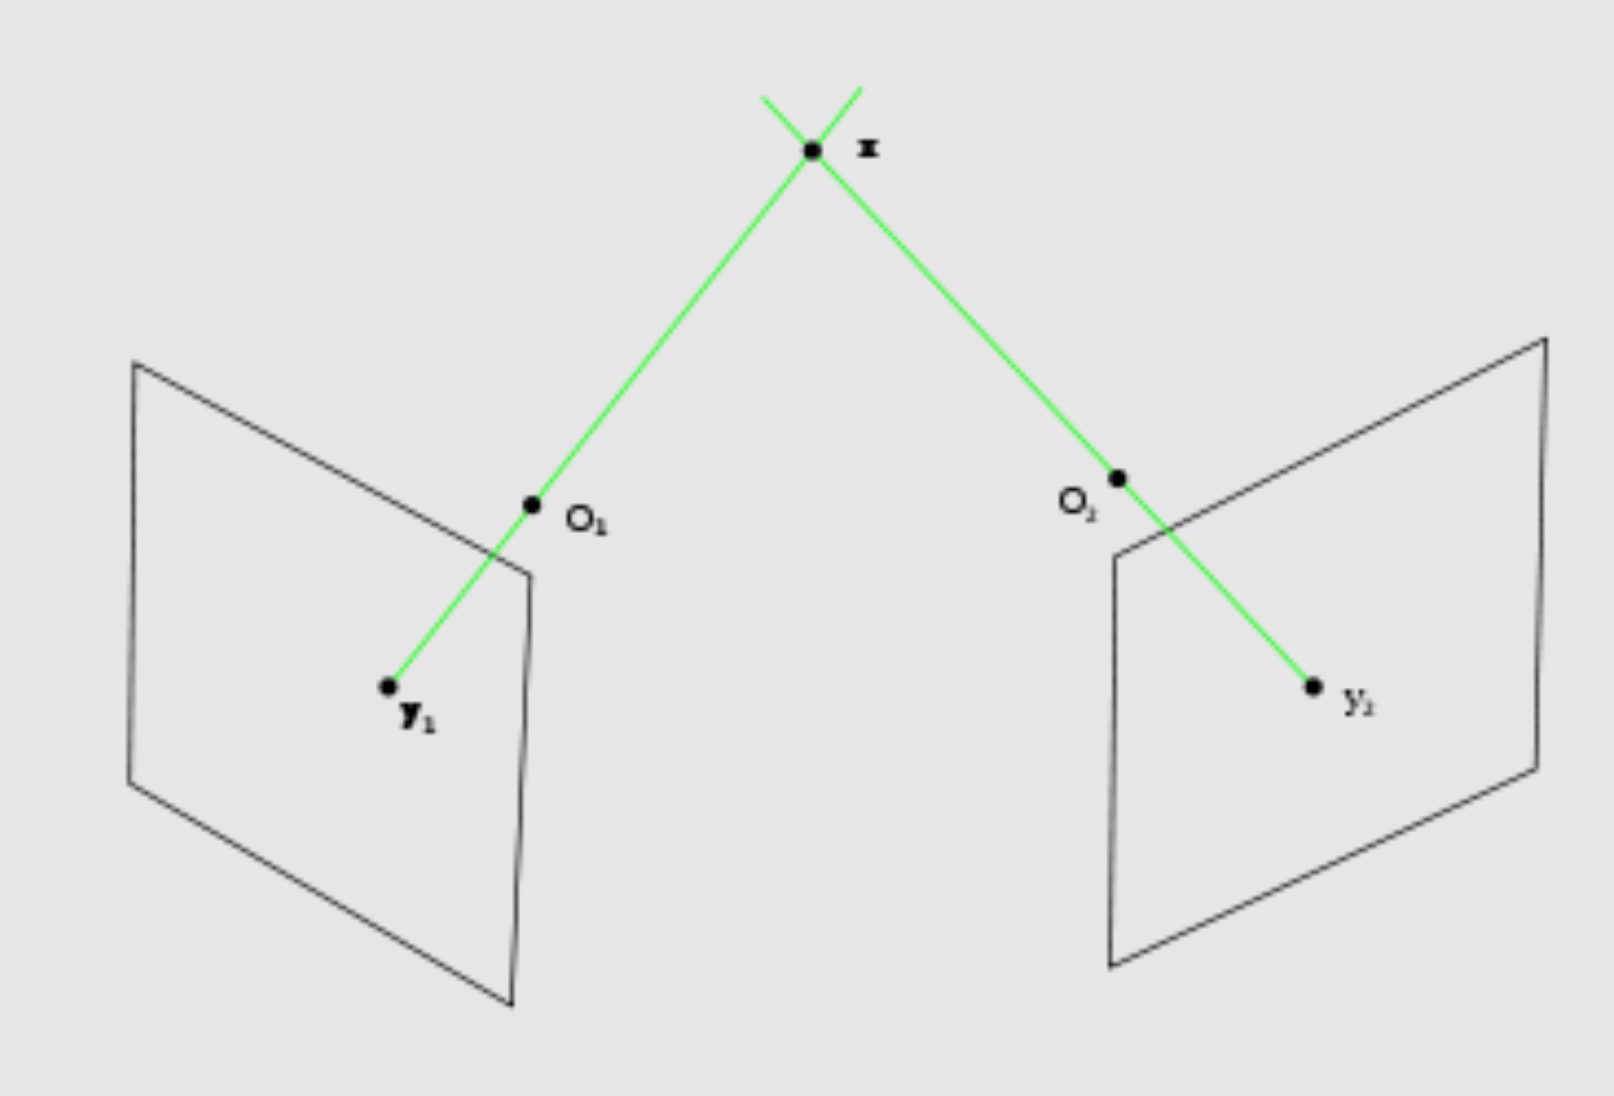
\includegraphics[height=4cm]{Res/Triangulation.png}


Der Grund warum die Pixel der „Schablone“ im Projektor zufällig angeordnet sind liegt darin, dass die unterschiedlichen lokalen Nachbarschaftsbedingungen die Pixelzuordnung zwischen dem statischen und dem dynamisch veränderten Bild erleichtern.


\subsection{Das Schattenproblem}

Aufgrund der Entfernung der verbauten RGB Kamera zur Infrarot Kamera weisen die Bilder beider Kameras einen kleinen Versatz auf.
Schatten im Tiefenbild entstehen aufgrund der Entfernung des Infrarotprojektors zur Infrarotkamera. Der Schatten im Muster macht es für den Sensor unmöglich die Tiefe festzustellen. Daher werden die Pixel in diesen Regionen auf den Wert 0 gesetzt.\\


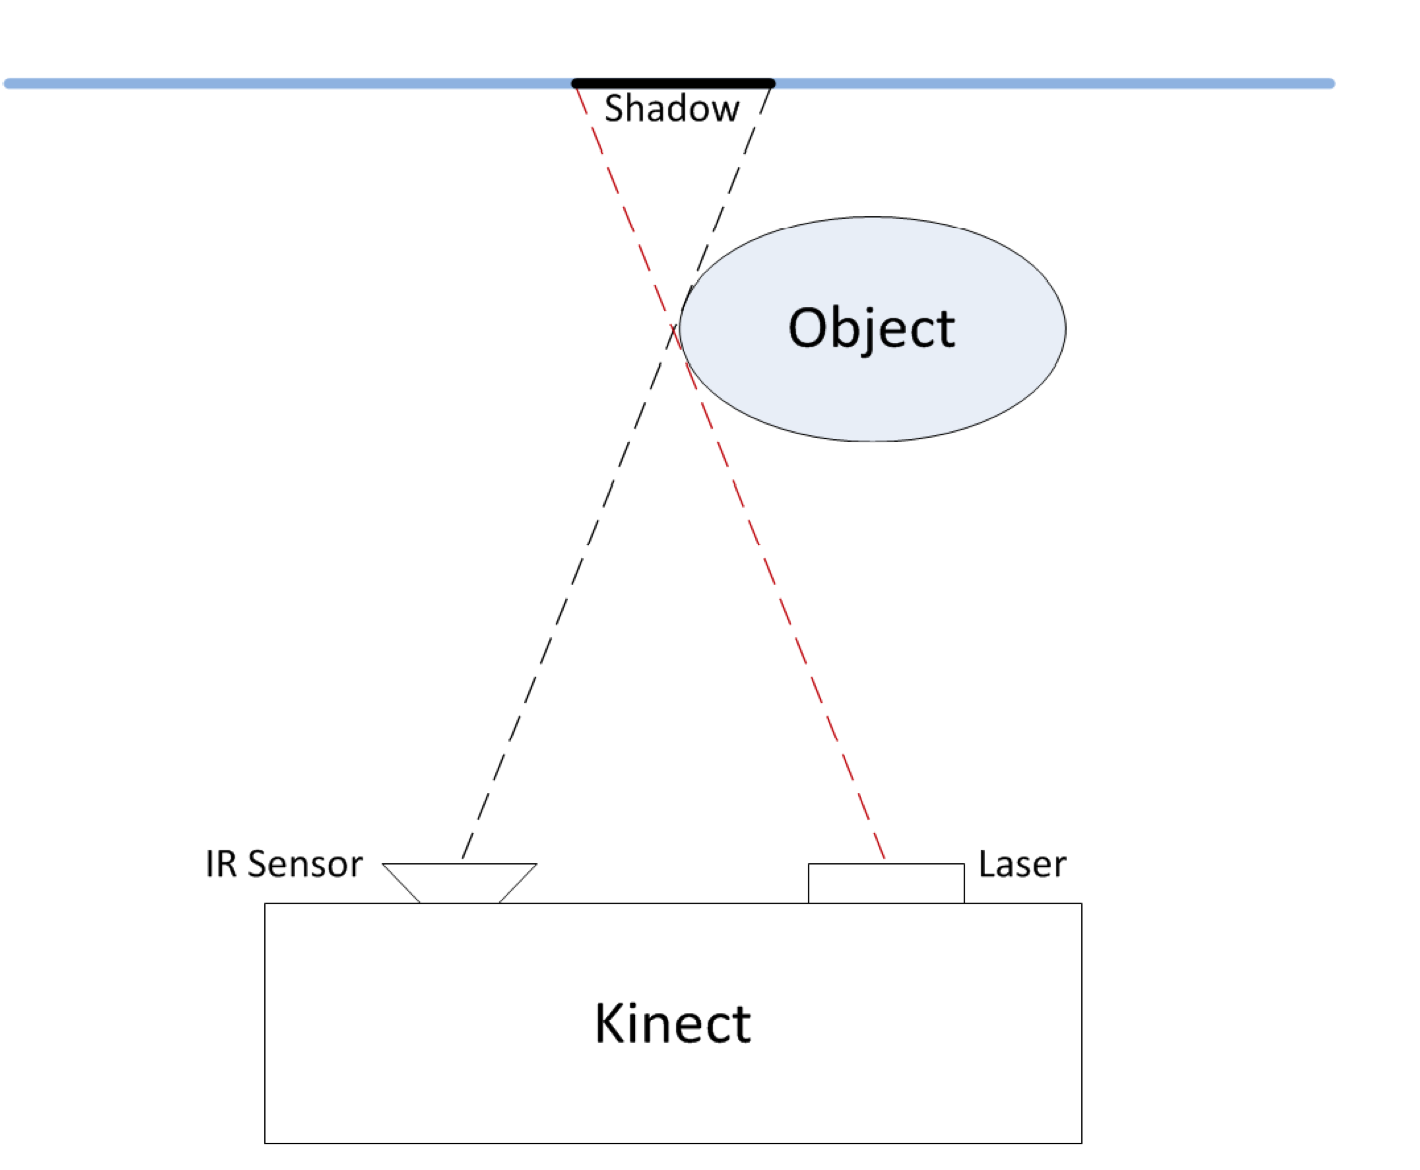
\includegraphics[height=4cm]{Res/Schatten_Strahl.png}


Das Objekt blockiert die Strahlen des Lasers. Da für die Tiefenberechnung das vom IR-Projektor emittierte Musters benötigt wird, ist es für die Kinect unmöglich die Distanz in Bereichen zu berechnen welche außerhalb der Erreichbarkeit des IR Strahlenmusters liegen. \\

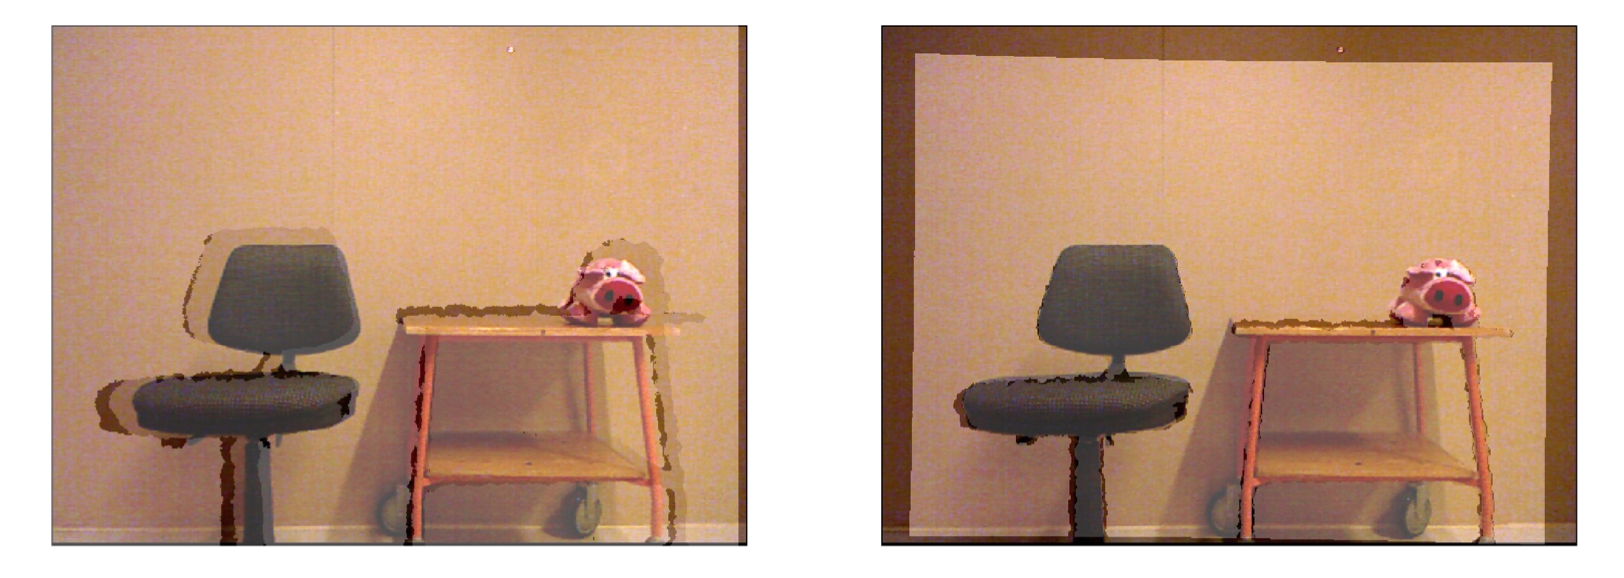
\includegraphics[height=4cm]{Res/Schatten.png}


Da der Infrarot Sensor links des Projektors positioniert ist, treten die Schatten auch linksseitig der Objekte auf. 

\chapter{Die Skelettierung}
\label{ch:Skelettierung}
\Autor{Sandra Schröder}\\\\
Unter einem Skelett versteht man einen Deskriptor, der die topologischen Eigenschaften eines Objekts beschreibt. Das sind Merkmale, die sich nicht explizit auf die konkrete Form einer Region beziehen, sondern auf ihre strukturellen Eigenschaften, die auch bei starken Verformungen erhalten bleiben. Zur Erfassung von bestimmten Eigenschaften von Binärbildern vereinfachen Skelette die Analysen, da durch die Reduzierung der Daten unwesentliche Eigenschaften ausgeblendet werden. Diese Abstraktion von für die Anwendung unwichtigen Eigenschaften ist eine zentrale Eigenschaft des Skelettes beziehungsweise eines Deskriptors im Allgemeinen. 
Historisch sind im Laufe der Entwicklung diverser Skelettierungsalgorithmen 
immer mehr konkrete Anforderungen an Skelette entstanden. \\
Eine wichtige Anforderung ist die  \emph{Konnektivität} des Skeletts. Dies bedeutet, dass es keine Lücken und Unterbrechungen im Skelett gibt, denn ein zusammenhängendes Objekt sollte ein zusammenhängendes Skelett besitzen.\\
Viele Skelettierungsverfahren fordern, dass ein Skelett genau ein Pixel breit ist. Dies ist beispielsweise in der Datenkomprimierung wichtig. Möchte man die Struktur eines
Objektes mit möglichst wenig Pixeln speichern, genügt ein
Skelett mit der minimal möglichen Pixelbreite. Eine breitere
Skelettlinie könnte unter Umständen zu viele unnötige Informationen beinhalten. Des Weiteren sollte das Skelett zentriert im Objekt liegen. Das bedeutet, dass Abstand der
Pixel der Skelettlinien nach links und nach rechts 
möglichst gleich sein sollte.\\
In wie weit alle Anforderungen an das Skelett erfüllt sein müssen, ist allerdings für jeden Anwendungfall neu zu diskutieren.
Dieses Kapitel beschreibt bekannte Konzepte und Verfahren zur Skelettierung im Bereich der Bildverarbeitung.
Zwei Verfahren wurden im Rahmen der Projektarbeit genauer untersucht: Die Skelettierung mittels \emph{Thinning} und mittels \emph{Distanztransformation}. \\
Um die Übersicht über die weiteren grundlegenden Verfahren und Konzepte zu vervollständigen, werden diese in einem separaten 
Abschnitt kurz vorgestellt.
\section{Skelettierung mittels Thinning}
\label{sec:thinning}
\Autor{Johannes Böhler, Christopher Kroll}\\ \\
Das Thinning bezeichnet eine Kategorie von Methoden zur Skelettierung von 2D sowie 3D Objekten. In dieser Projektarbeit ist der Fokus ausschlie"slich auf die 2D Skelettierung gerichtet, da die Kinect kein vollkommenes 3D Modell eines Objektes liefert. Sie erfasst das Objekt lediglich aus einem Blickwinkel, desshalb erhält man nur ein 2,5 dimensionales Modell. Es werden nur Tiefeninformationen bezüglich der Seite des Objektes, welche der Kinect zugewendet ist bereitgestellt. Die  Tiefeninformationen der Rückseite bleiben verborgen. Um ein vollständiges 3D Modell zu erhalten müssten mindestens 2 Kinects verwendet werden und die Informationen beider Geräte zusammengeführt und vereinheitlicht werden. \\ \\
Alle Thinning-Algorithmen verbindet das iterative Abtragen des Musters oder der Oberfläche. Dabei werden nach und nach die Konturpixel, also die Objektpixel, die mit den Hintergrundpixeln benachbart sind, "uberpr"uft. Je nach Algorithmus liegen verschiedene Kriterien vor, ob diese gel"oscht, also als Hintergrundpixel markiert werden k"onnen. Ein Kriterium ist auf jeden Fall, dass die Zusammengeh"origkeit der Skelettpixel bewahrt wird. Eine weitere Gemeinsamkeit der unterschiedlichen Ans"atze ist, dass das Ausd"unnen solange stattfindet, bis am Objekt keine "Anderung mehr gemacht wurde.

Beim Thinning wird die Zusammengeh"origkeit nicht ver"andert, wodurch die topologische Struktur des Objektes erhalten bleibt. 

\subsection{A Fast Parallel Algorithm for Thinning Digital Patterns} 
\Autor{Johannes Böhler}\\\\
\label{subsec:fastparallel}
Der gesamte Algorithmus erstreckt sich über mehrere Iterationen. Die Randpixel des Musters werden Schicht für Schicht abgetragen. Die Iterationen selbst, sind wiederum in zwei Subiterationen unterteilt. Das Abtragen der „Schichten“ wird somit in zwei unterschiedliche Phasen aufgespalten.
Mit Hilfe der ersten Subiteration werden sowohl Süd- und Ostgrenzpunkte als auch Nordwest Eckpunkte entfernt. Das entfernen von Nord- und Westgrenzpunkten sowie von Südosteckpunkten erfolgt in der zweiten Subiteration.
\begin{figure}[!ht]
        \centering
        \begin{subfigure}[b]{0.3\textwidth}
                \centering
                 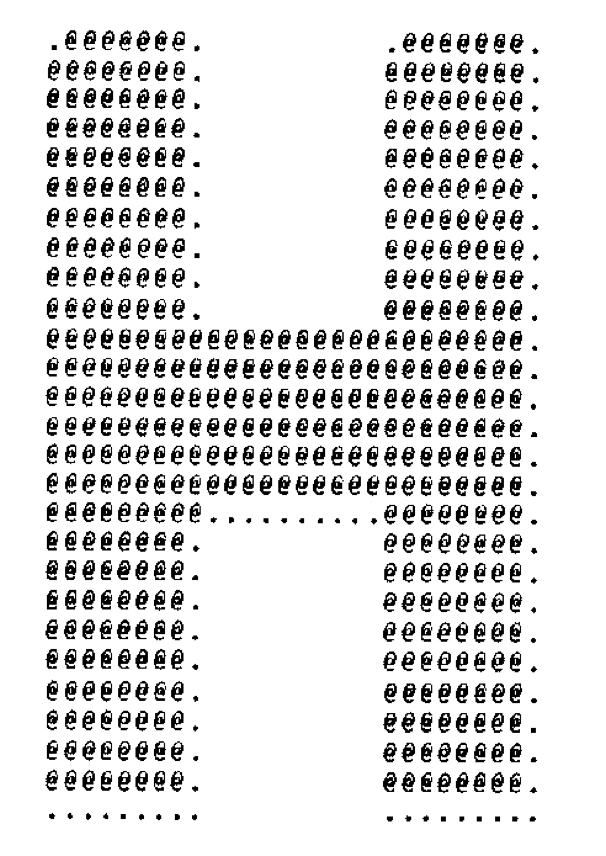
\includegraphics[height=5cm]{Res/SuedOst.png}
                \caption{Nach erster Subiteration (zu Beginn)  }
               
        \end{subfigure}%
        ~ %add desired spacing between images, e. g. ~, \quad, \qquad etc.
          %(or a blank line to force the subfigure onto a new line)
        \begin{subfigure}[b]{0.3\textwidth}
                \centering
                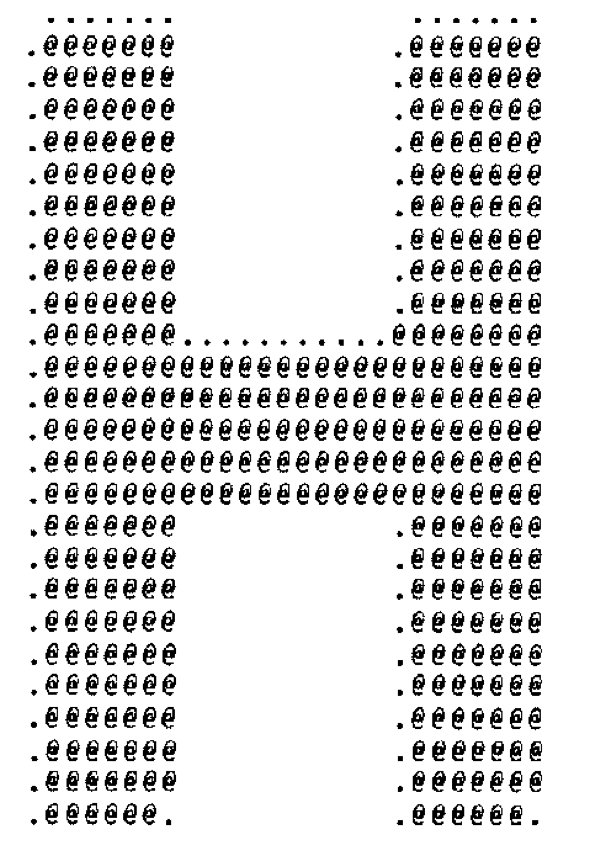
\includegraphics[height=5cm]{Res/NordWest.png}
                \caption{Nach zweiter Subiteration (zu Beginn)}
               
        \end{subfigure}
        ~ %add desired spacing between images, e. g. ~, \quad, \qquad etc.
          %(or a blank line to force the subfigure onto a new line)
        \begin{subfigure}[b]{0.3\textwidth}
                \centering
                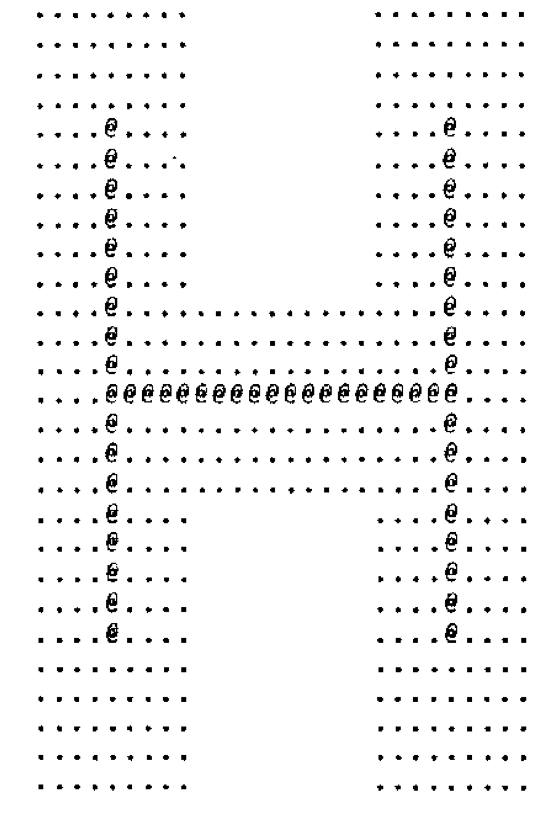
\includegraphics[height=5cm]{Res/Skelett.png}
                \caption{Skelett des Ursprungsmuster}
               
        \end{subfigure}
        \caption{Zustände des Algorithmus}
\end{figure}

\subsubsection{Anforderungen an den Algorithmus}

\begin{itemize}
\item[-] Das Rauschen, welches der Algorithmus verursacht soll so gering wie möglich gehalten werden.
\item[-] Das Skelett des Ursprungsmusters soll die Endpunkt- und Pixelverbundenheit erhalten.
Endpunktverbundenheit bedeutet, dass sich zwischen zwei Endpunkten eines Skeletts keine unverbundenen Stellen befinden.
\item[-] Das Skelett soll nach Durchlaufen des kompletten Algorithmus in einheitlicher Dicke von einem Pixel vorliegen.
\item[-] Der Algorithmus soll möglichst schnell und effizient arbeiten um Echtzeitfähigkeit gewährleisten zu können. \\
\end{itemize}

\subsubsection{Ablauf des Algorithmus}

Es wird davon ausgegangen, dass zu Beginn ein binär digitalisiertes Bild vorliegt.
Die Pixel werden mit Hilfe einer zweidimensionalen Matrix IT durchlaufen, deren Wert an der jeweiligen Stelle IT(i,j) entweder 0 oder 1 ist.
Mit Muster ist die Menge an Pixeln gemeint, welche den Wert eins haben.
Es werden in Abhängigkeit von den 8 Nachbarpixeln (siehe Abbildung 4.5), Transformationen auf den betrachteten Pixel P1 angewendet. Dieser Vorgang wird iterativ auf die Matrix IT angewendet.

Der neue Wert eines Pixels während der n-ten Iteration hängt von dem eigenen Wert während der (n-1)ten Iteration und den Werten der acht Nachbarn während der (n-1)ten Iteration ab. Dies ermöglicht paralleles Transformieren mehrerer Bildpunkte. 
Die Bedingungen, welche zum Ausführen der Transformation erfüllt sein müssen werden über ein 3x3 Pixel Fenster abgefragt. Der Punkt P1 über dessen Transformation entschieden wird, ist mit allen acht Nachbarn direkt verbunden.\\
\begin{figure} [!ht]
\centering
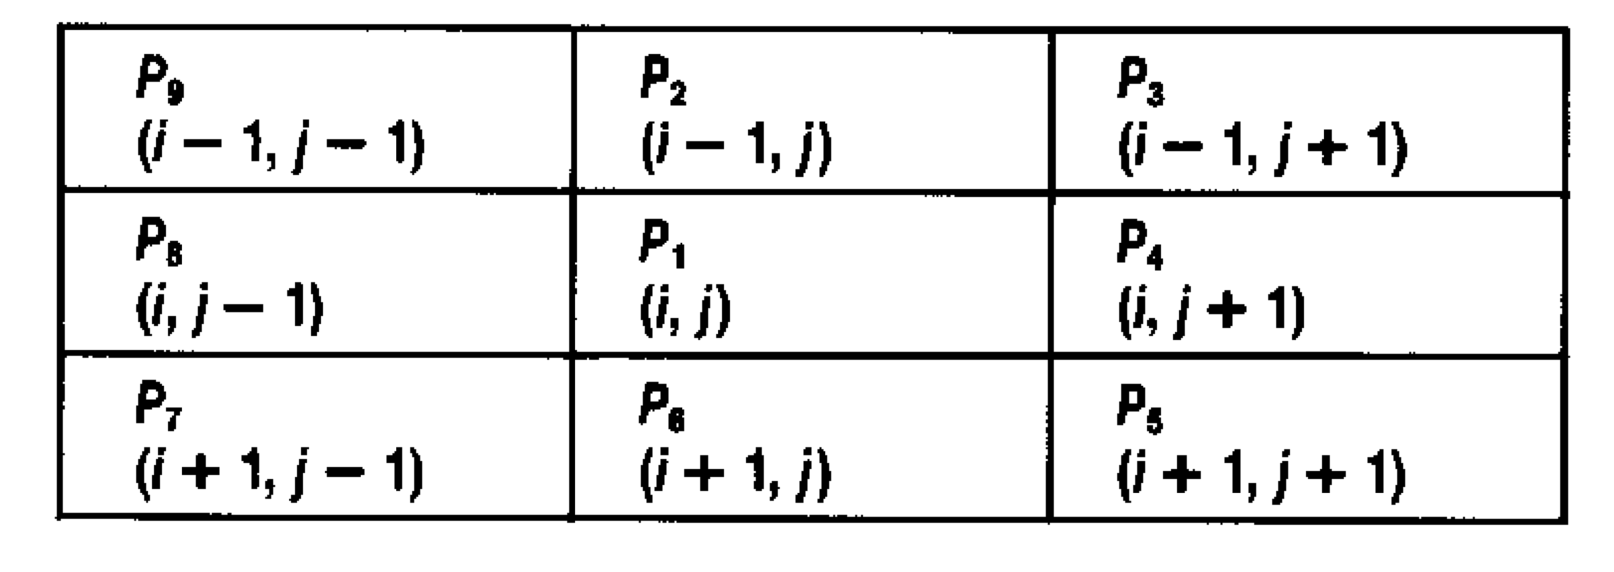
\includegraphics[width=0.7\linewidth]{./Res/PixelNachbarschaft}
\caption{Betrachteter Pixel P1 und Nachbarumgebung}
\label{fig:PixelNachbarschaft}
\end{figure}

Der Algorithmus entfernt alle Randpunkte des Musters, außer den Pixeln welche Bestandteil des Skeletts sind. Um die Verbundenheit des Skeletts zu gewährleisten wird ein  Iterationsschritt in zwei Subiterationen aufgeteilt.\\\\
In der ersten Subiteration wird der Punkt P1 aus dem Muster gelöscht, wenn er folgende Bedingungen erfüllt:
\begin{itemize} 
\item \emph{a)} 2<=B(P1)<=6     
B entspricht der Anzahl der Nachbarn von P1 !=0
Die Anzahl der Nachbarn von P1 welche den Wert 1 haben, muss somit zwischen 2 und 6 liegen.
\item \emph{b)}  A(P1)=1
Anzahl der „01“-Folgen 
Die Anzahl der 01 Folgen in der geordneten Folge P2,P3...P9 muss genau eins betragen.
\item \emph{c)}  P2*P4*P6=0  
Mindestens ein Pixel der Pixelmenge P2, P4, P6 muss den Wert Null haben.
\item \emph{d)}  P4*P6*P8=0
Mindestens ein Pixel der Pixelmenge P4, P6, P8 muss den Wert Null haben.
\end {itemize}
Sind alle Bedingungen a, b ,c und d erfüllt so wird der Wert des Pixels auf 0 gesetzt.
Dies bedeutet dass er kein Teil des Skelett-Musters mehr ist.
Wird eine der Bedingungen nicht erfüllt, so bleibt der Pixelwert bei 1.\\
\begin{figure}[!ht]
  \centering
  \makebox[\textwidth]{%
   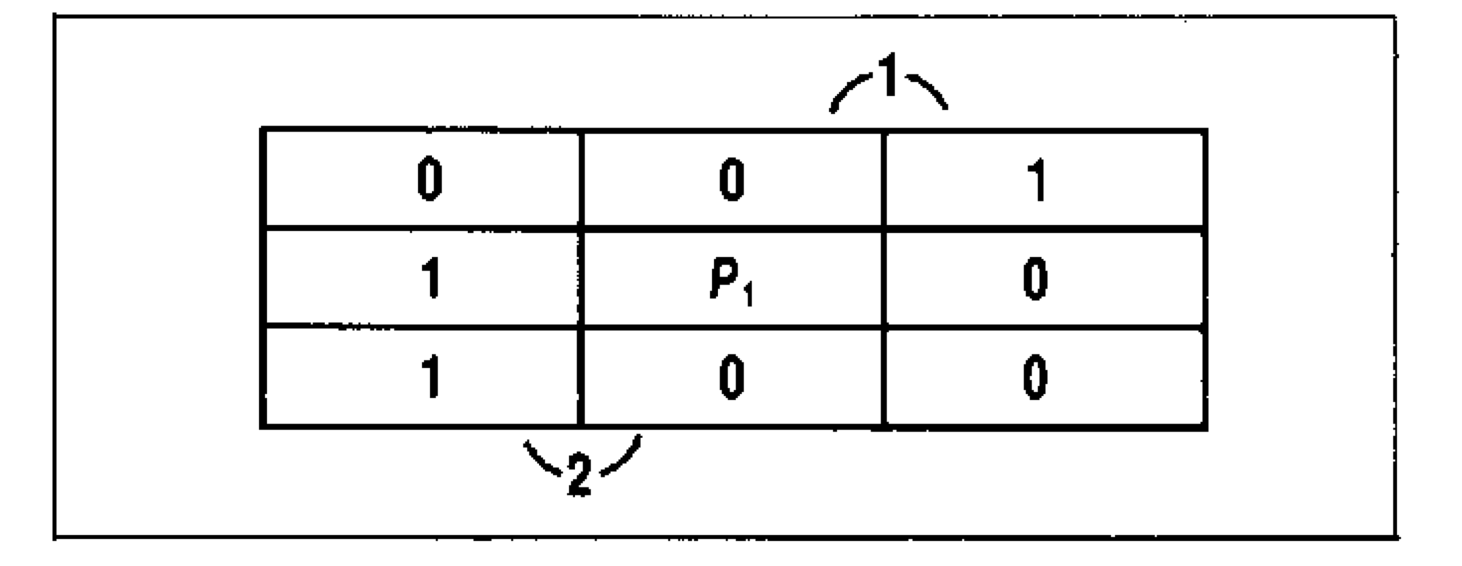
\includegraphics[width=8cm]{Res/01Folgen.png}
  }
   \caption{Bedingung B: Anzahl 01 folgen in zyklischer Reihenfolge  }
\end{figure}

In der zweiten Subiteration wird P1 gelöscht falls folgende Bedingungen gelten:
\begin{itemize} 
\item \emph{a)}  2<=B(P1)<=6 
\item \emph{b)}  A(P1)=1 
\item \emph{c)}  P2*P4*P8=0 
\item \emph{d)}  P2*P6*P8=0
\end{itemize}

Nur die Bedingungen c und d haben sich geändert.\\
Um die Bedingungen der ersten Subiteration zu erfüllen, muss
P4=0 oder P6=0 oder (P2=0 und P8=0)  erfüllt sein.
Dies impliziert dass P1 entweder Süd- oder Ost-Grenzpunkt, oder Nordwesteckpunkt ist.Um die Bedingungen der zweiten Subiteration zu erfüllen muss
P2=0 oder P8=0 oder (P4=0 und P6=0) sein.
P1 ist Nord- oder West-Grenzpunkt oder Südosteckpunkt.\\

\begin{figure}[!ht]
  \centering
  \makebox[\textwidth]{%
   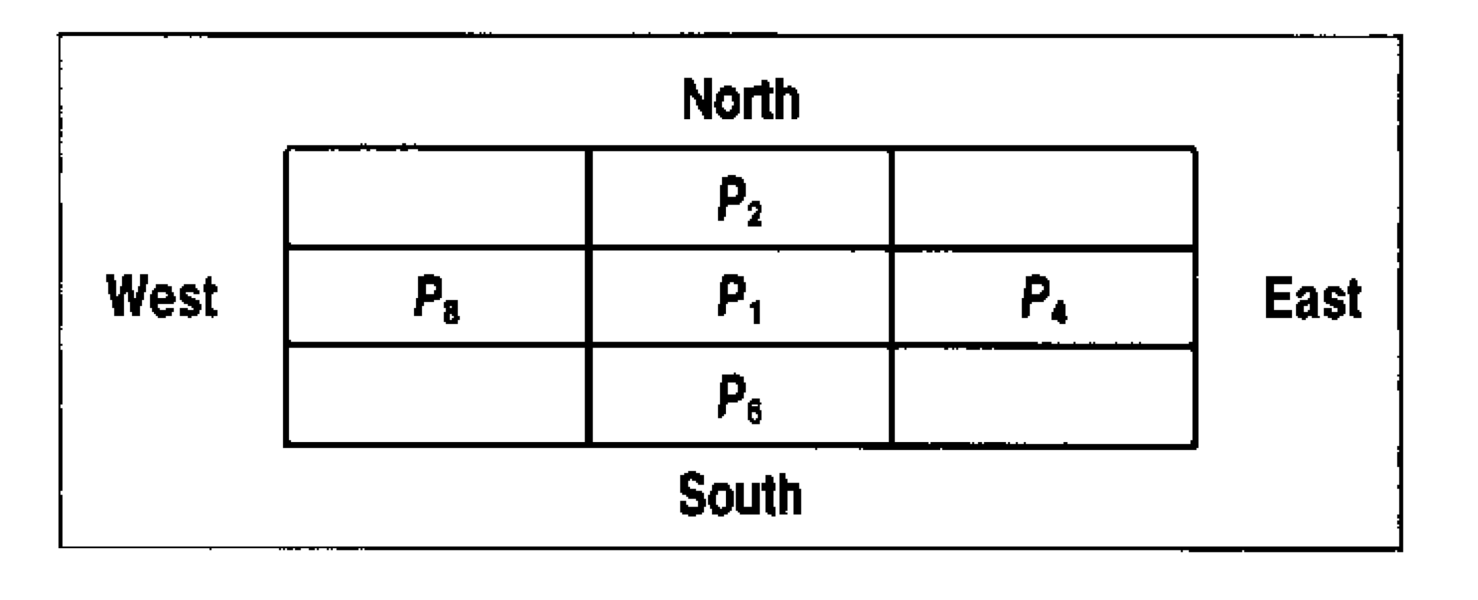
\includegraphics[width=8cm]{Res/Orientierung.png}
  }
   \caption{Betrachteten Nachbarpunkte in den Bedingungen c und d  }
\end{figure}




Während mit Bedingung A (2<=B(P1)<=6) die Endpunkte des Skeletts erhalten werden, so wird mit Bedingung B (A(P1)=1) die Auslöschung von Punkten zwischen den Endpunkten der Skelettlinie verhindert.\\

\begin{figure}[!ht]
  \centering
  \makebox[\textwidth]{%
  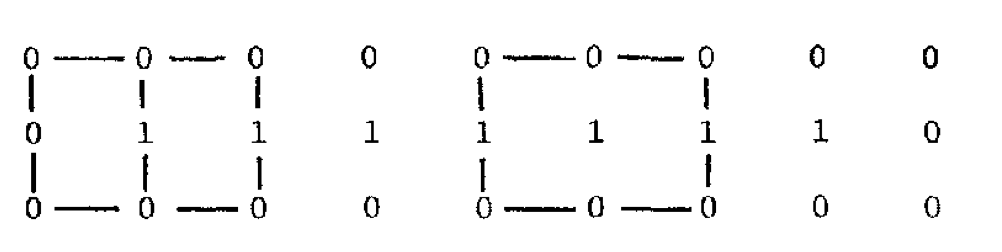
\includegraphics[width=8cm]{Res/EndpktVerbheit.png}
  }
   \caption{Gewährleistung der Pixelverbundenheit}
\end{figure}


In der Matrix Search M befinden sich während der ersten Iteration alle Pixel die gelöscht werden dürfen, da sie den Bedingungen der ersten Iteration genügen. Ist dies nicht der Fall, so ist der Counter=0 und der Algorithmus beendet, da es keine zu löschenden Pixel mehr gibt. Die Skelettierung ist somit beendet.

Falls der Counter ungleich null ist, werden die Pixel welche den Bedingungen genügen von der Matrix IT (Skelett-Muster) abgezogen, der Counter wird null gesetzt und es wird zur zweiten Iteration fortgeschritten. Dort findet der Ablauf mit veränderten Bedinungen c und d wiederholt statt. Ist der Counter auch nach dem Durchlaufen der zweiten Subitertation ungleich null so wird der Vorgang iterativ fortgeführt.\\ \\ \\ \\ \\ \\ \\ \\ \\ \\ \\ \\

<<<<<<< HEAD
\begin{figure}
\centering
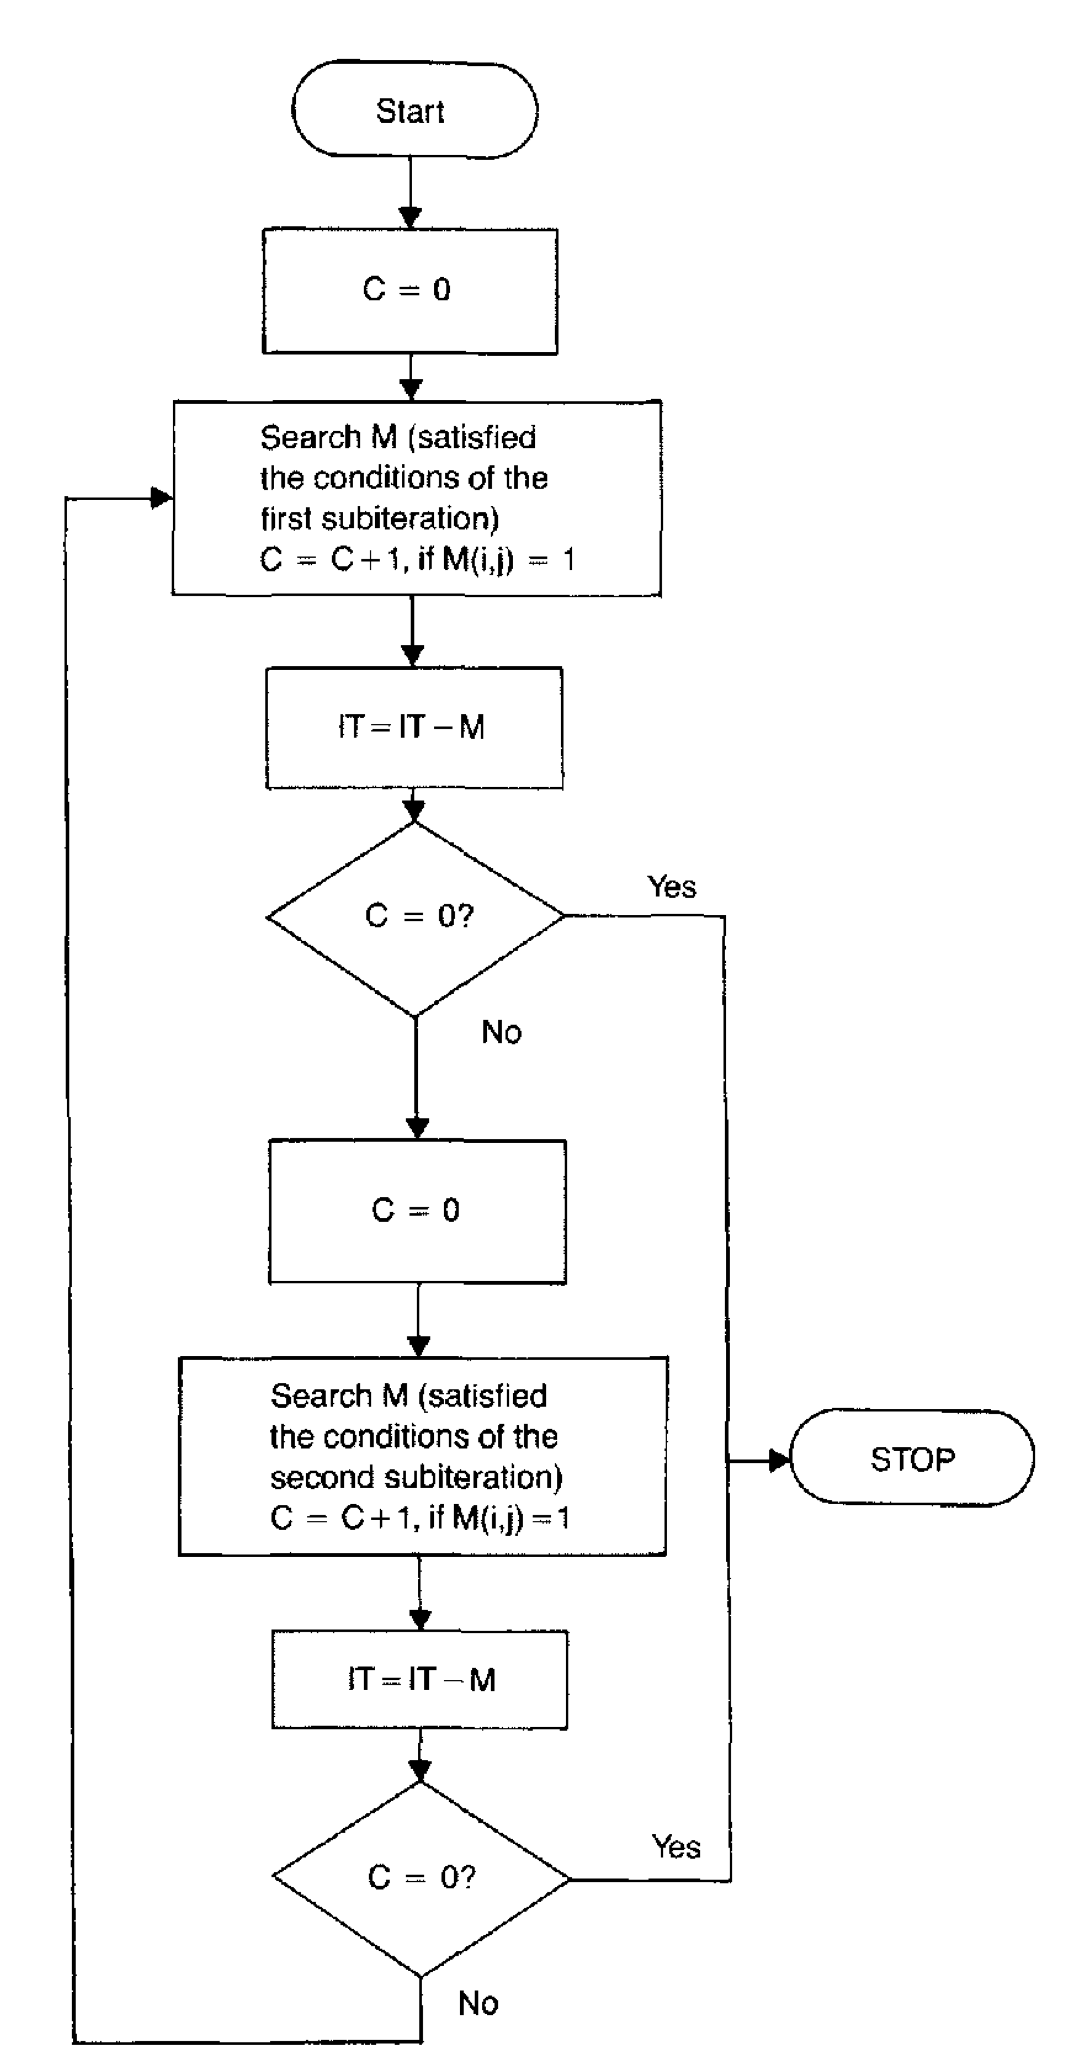
\includegraphics[width=0.7\textwidth]{./Res/AlgUebersicht}
\caption{Gesamter Algorithmus in der Übersicht}
\label{fig:AlgUebersicht}
=======

\begin{figure}[!ht]
  \centering
  \makebox[\textwidth]{%
  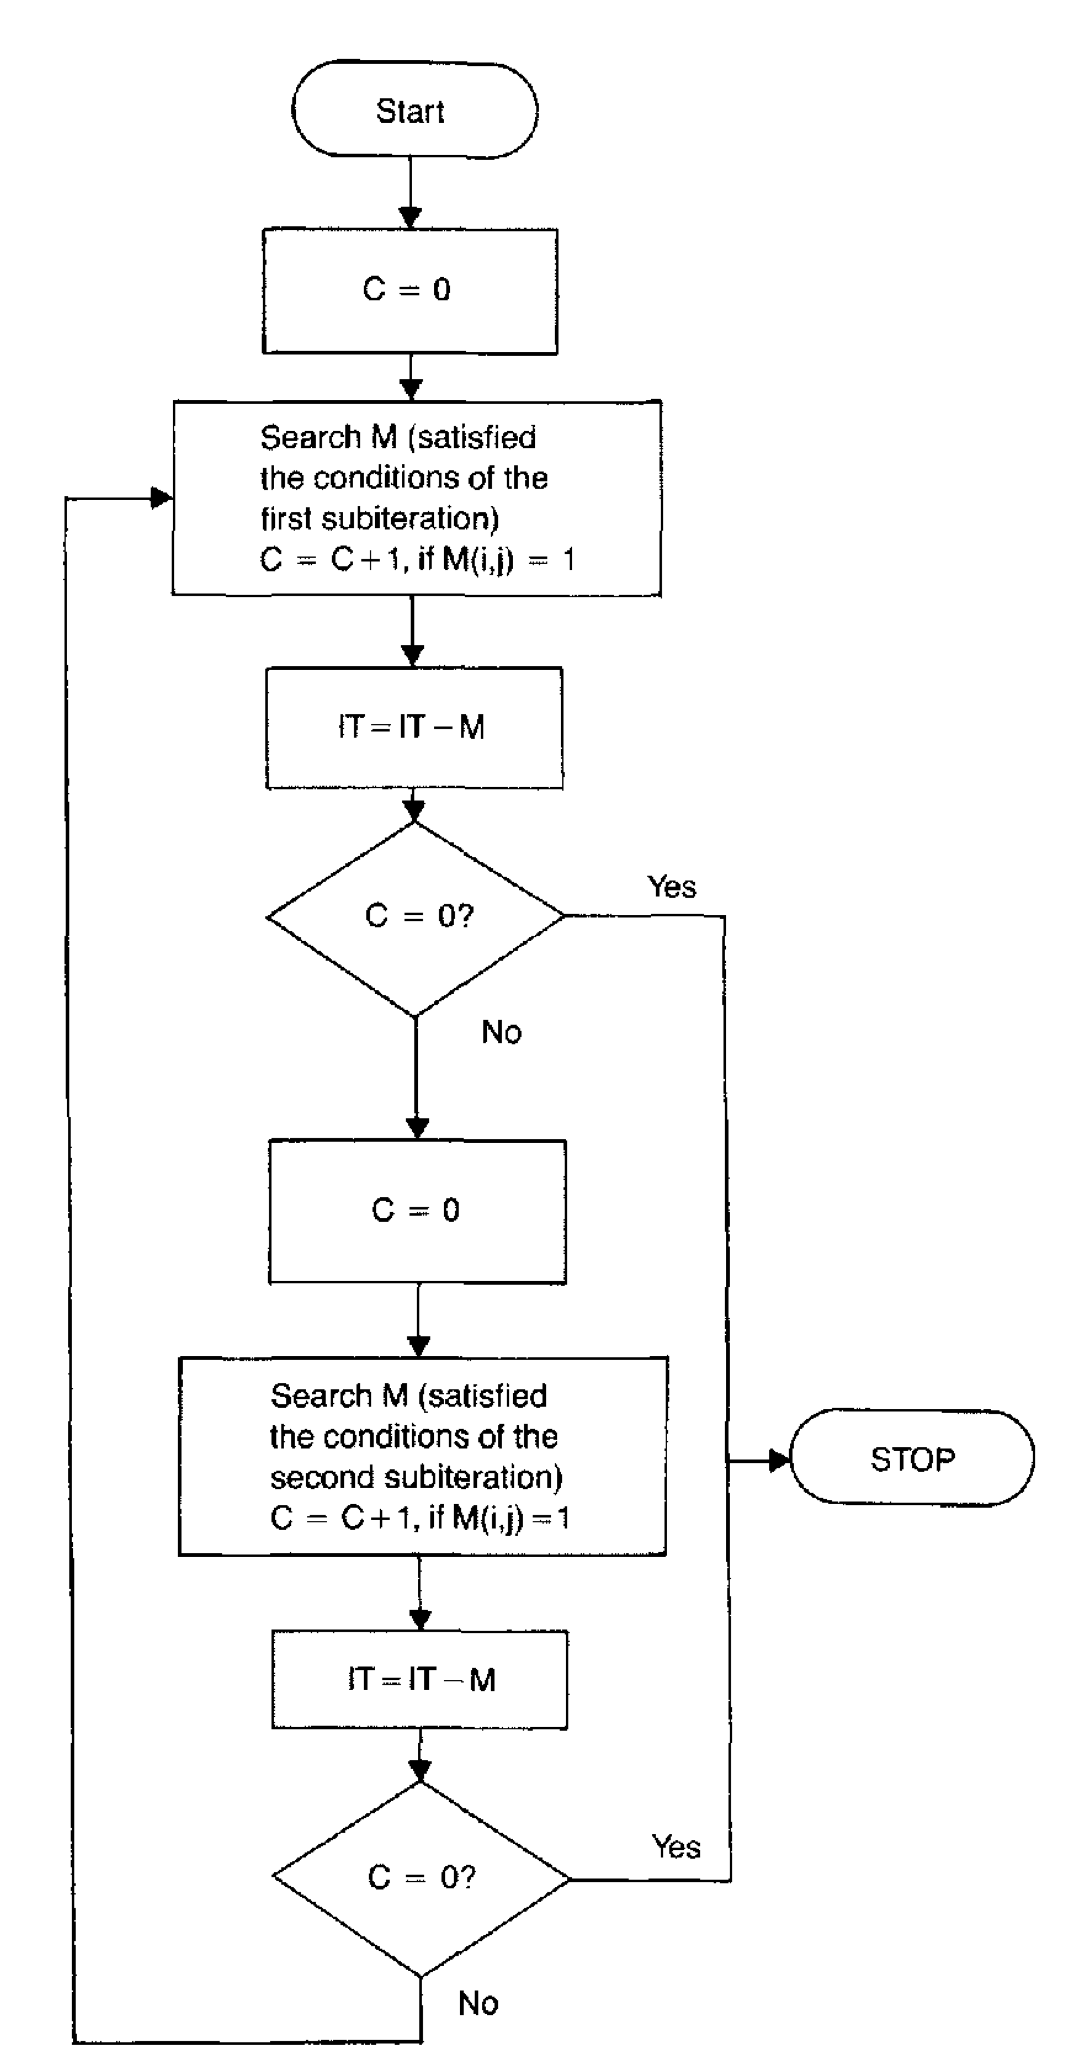
\includegraphics[width=8cm]{Res/AlgUebersicht.png}
  }
   \caption{Gesamter Algorithmus in der Übersicht}
>>>>>>> Korrekrur schrift
\end{figure}
\FloatBarrier
\subsubsection{Resultate}

<<<<<<< HEAD
Der Algorithmus erzielt sehr gute Ergebnisse im Bezug auf Verbundenheit und Rauschverhalten der Randpunkte. Die Bedingungen welche zum Auffinden der zu löschenden Randpunkte führen sind sehr simpel. Durch den Bezug auf die n-1te Iteration zur Abfrage der Bedingungen kann der Algorithmus sehr schnell ausgeführt werden, da keine Warteabhängikeiten bestehen. \\ \\
Nach dem Auseinandersetzen mit dem Algorithmus entschied man sich diesen auch zu implementieren.
=======
Der Algorithmus erzielt sehr gute Ergebnisse im Bezug auf Verbundenheit und Rauschverhalten der Randpunkte. Die Bedingungen welche zum Auffinden der zu löschenden Randpunkte führen sind sehr simpel. Durch den Bezug auf die n-1te Iteration zur Abfrage der Bedingungen werden Warteabhängigkeiten vermieden und ein performantes Verarbeiten der Bildpixel gewährleistet.
>>>>>>> Korrekrur schrift

\newpage
\section{Skelettierung mittels Distanztransformation}
\label{sec:distanztransformation}
\Autor{Sandra Schröder}\\\\
Die Distanztransformation eines Binärbildes enthält Informationen über den Abstand der Objektpixel zum Hintergrund. Der Abstand zum Hintergrund wird für jeden Objektpixel bestimmt und in einem
weiteren Bild (gleiche Dimension und Größe wie das Binärbild) als Grauwert an der Stelle des Objektpixels gespeichert. Das Ergebnis ist die sogenannte \emph{Distance Map} (Abbildung \ref{fig:distance_map_beispiel}). \\
Zur Bestimmung des Abstands benötigt man Metriken. Eine gängige Metrik - die für den Algorithmus im Rahmen dieser Arbeit auch genutzt wurde - ist die euklidische Metrik $d_2$:
\begin{equation}
\label{eq:d2}
d_2(p,q) = \sqrt{(p_x - q_x)^2 + (p_y - q_y)^2}  
\end{equation}
Die Definition einer Nachbarschaft spielt
ebenfalls eine Rolle. Wählt man eine
4er-Nachbarschaft, wird der Abstand vom Objektpixel zur linken und zur rechten Seite, sowie nach oben und nach unten berechnet. Man erhält dementsprechend
vier Abstände. In der Distance Map wird der minimale Abstand von den vier Werten gespeichert. Bei einer 8er-Nachbarschaft
kommen die diagonalen Richtungen dazu. Abhängig von der gewählten
Nachbarschaft und der Metrik ergeben sich unterschiedliche Distance
Maps.\\\\
Die Pixel mit dem größten Abstand zum ersten Pixel des Hintergrunds sind die hellsten Pixel in der Distance Map. Die umgebenden Pixel haben einen kleineren Grauwert und der Grauwert der Pixel verringert sich, je näher die Pixel am Hintergrund liegen.
Dementsprechend beschreiben die hellsten Pixel des \emph{Grauwertgebirges} eine skelettförmige Struktur, die im Folgenden aus der Distance Map extrahiert werden soll.
Wir verfolgen einen Ansatz, der auf der Bildung des Gradienbetrages der Distance Map beruht.\\
\begin{figure}[h]
	\centering
	\begin{minipage}{4cm}
		\centering
		
\includegraphics[width=1.0\linewidth]{./fig/person.jpg}
		\label{fig:beispiel_person}
	\end{minipage}
	\hspace{3cm}
	\begin{minipage}{4cm}
		\centering
		
\includegraphics[width=1.0\linewidth]{./fig/distance_map_beispiel}	
	\end{minipage}
	\caption{Beispiel einer Distance Map. Links: Originalbild. Dieses wurde zuerst invertiert, damit das Objekt (Person) weiß markiert ist. Rechts: Resultat der Distanztransformation. Aufällig ist das Maximum in der Mitte.}
	\label{fig:distance_map_beispiel}
\end{figure}
Ein Graubild kann als skalare Funktion $f(x,y)$ beschrieben werden mit $x,y \in \mathbb{N}$ und
$0 \leq f(x,y) \leq 255$. 
Die Idee ist, den Gradienten beziehungsweise den Gradientenbetrag der Distance Map zu bestimmen. Der Gradient (Gleichung \ref{eq:gradient}) ist ein Differentialoperator und liefert, angewandt auf ein Skalarfeld, die Richtung des stärksten Anstiegs, sowie die Amplitude des Anstiegs (Gradientenbetrag):
\begin{equation}
\label{eq:gradient}
%      \[
   grad(f(x,y)) = \nabla f(x,y) = \begin{bmatrix}
         \frac{df}{dx}        \\[0.3em]
         \frac{df}{dy} \\[0.3em]
      \end{bmatrix}
%  \]
\end{equation}
Entsprechend der Definition des Gradienten, ist an den lokalen Maxima des Grauwertgebirges der Gradientenbetrag gleich null.\\
Speichert man den Gradientenbetrag ebenfalls als Grauwertbild mit gleicher Dimension und Größe wie die Distance Map, wird der Gebirgskamm als Linie mit kleinen Grauwerten (fast Null) kodiert. Diese markiert das Skelett. Eine schwellwerbasierte Segmentierung des Gradientenbetragbildes bewirkt, dass die Skelettlinien schwarz sind (Abbildung \ref{fig:bildung_gradient}). Andere Bereiche, die größer als der Schwellwert sind und somit nicht zum Skelett gehören, erhalten den Grauwert $255$ (weiß). 
\begin{figure}
\centering
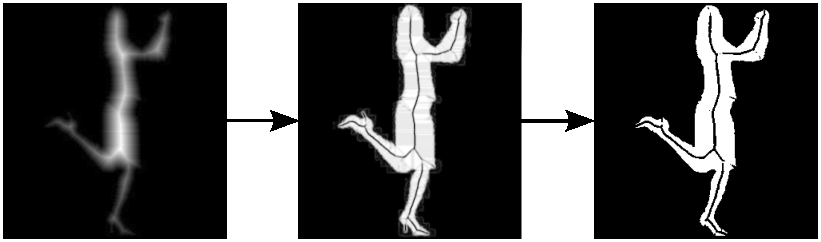
\includegraphics[width=1.0\linewidth]{./fig/bildung_gradient}
\caption{Segmentierung des Gradientenbetrags aus der Distance Map. Von links nach rechts: Distance Map, Gradientenbetrag der Distance Map, Segmentiertes Gradientbetragsbild}
\label{fig:bildung_gradient}
\end{figure}
\FloatBarrier
\noindent
Um endgültig nur die Skelettlinie zu erhalten, wird die Differenz
zwischen der Distance Map und dem segmentierten Gradientenbetragsbild gebildet. Der Teil der Distance Map der nicht
auf der höchsten Stelle des Grauwertgebirges liegt, hat entweder einen Grauwert kleiner oder gleich $255$. Bei
der Differenzbildung kann der Grauwert dieser Pixel nur kleiner gleich 0 werden, da von diesen Grauwerten der Grauwert $255$ abgezogen wird (weißer Bereich des segmentierten Gradientenbetragsbildes). Negative
Grauwerte werden auf $0$ gesetzt. Als Ergebnis erhält man die Skelettlinie mit Grauwerten ungleich $0$. Um ein binärkodiertes Skelett zu erhalten, wird auf dem Differenzbild
anschließend eine schwellwertbasierte Segmentierung ausgeführt (Abbildung \ref{fig:differenzbildung}).
\begin{figure}
\centering
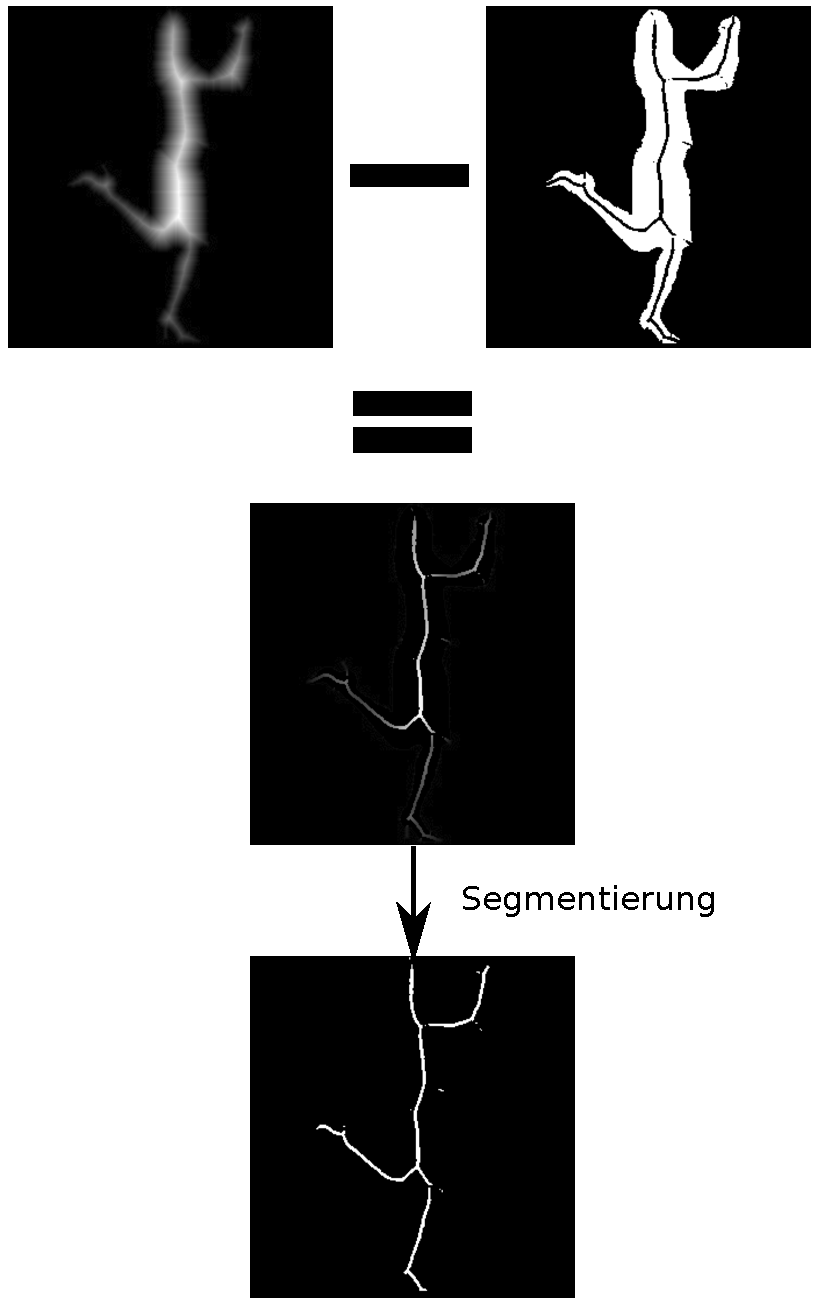
\includegraphics[width=0.8\linewidth]{./fig/differenzbildung}
\caption{Differenzbildung zwischen dem segmentieren Gradientenbetragsbild und der Distance Map.}
\label{fig:differenzbildung}
\end{figure}
Im Folgenden wird das aus der Distanztransformation bestimmte Skelett zur Abgrenzung zum Thinning-Algorithmus als \emph{Distanzskelett} bezeichnet.
\FloatBarrier
%\begin{figure}
%\centering
%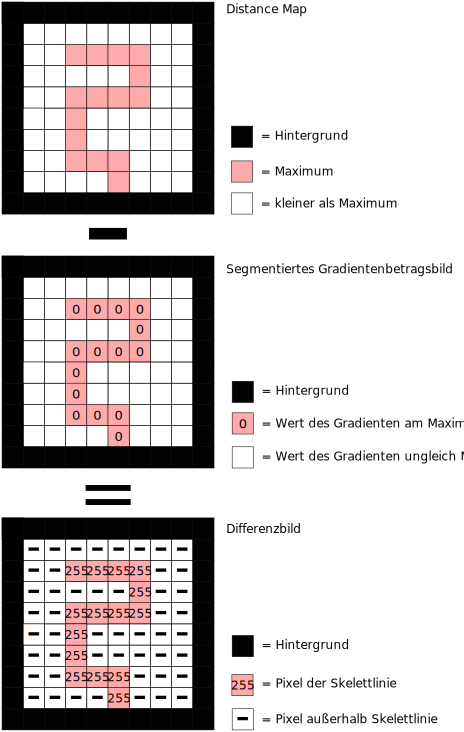
\includegraphics[width=1.0\linewidth]{./fig/skelettierung-prinzip}
%\caption{Die Idee der Skelettierung mittels Distanztransformation.}
%\label{fig:skelettierung-prinzip}
%\end{figure}
\clearpage
\subsection{Verwandte Arbeit \cite{extracting_skeletons_distancemaps}: Extracting Skeletons From Distance Maps}
\label{subsec:distancemap_verwandt}
\Autor{Sandra Schröder}\\\\ 
Zur oben beschrieben Berechnung des Skelettes aus einer Distance Map gibt es verwandte Arbeiten, von denen nun eine vorgestellt wird. 
In dem Paper \emph{Extracting Skeletons from Distance Maps} beschreibt der Autor einen Algorithmus, der effizient und schnell
aus einem distanztransformierten Bild ein Skelett extrahiert \cite{extracting_skeletons_distancemaps}. Der Autor legt besonders hohen Wert darauf, dass die Extraktion keine komplizierten Berechnungen beinhaltet. Er möchte vor allem auf die Berechnung
von Ableitungen höherer Ordnung und die Auswertung von komplexen Gleichungen verzichten. Das Verfahren, welches der Autor zur 
Extraktion der Skelettlinien eines Objekt vorstellt, ist die sogenannte \emph{Ridge Point Detection} (deutsch: \emph{Gebirgskammdetektion}). Dabei nutzt der Autor eine grundlegende Eigenschaft der Distance Map. Wie in Abschnitt \ref{sec:distanztransformation} beschrieben, ist die Distance Map ein Grauwertgebirge, wobei der Gebirgskamm zentriert im Objekt liegt. Betrachtet man nur diesen Teil der Distance Map und projiziert ihn auf das Originalbild, 
ist eine skelett-artige Beschreibung des Objekts zu erkennen.\\\\
Die Gebirgskammdetektion ist ein gradientenbasiertes Verfahren. Der Gradient zeigt nach Definition in die Richtung des stärksten Anstiegs (Gleichung \ref{eq:gradient}). Dies bedeutet, dass der Gradient eines Punktes, der nicht auf dem Kamm liegt, in die Richtung des Kammes zeigt. Wählt man nun Punkte näher am Kamm, so wird der Anstieg
geringer, da die Differenz zwischen dem Grauwert des betrachteten Gebirgspunktes und dem aktuell gewählten Punkt kleiner wird. Überquert man den Kamm, kehrt sich die Richtung des Gradienten um und zeigt wieder zum Kamm. Hier findet ein Vorzeichenwechsel des Gradientenbetrags statt. Der Punkt auf dem Gebirgskamm bildet eine \emph{sign barrier} zwischen den Gradientenbeträgen der sich gegenüberliegenden Punkte, wobei sich der dieser Punkt zwischen den beiden Punkten befindet. Diese
Beobachtung ist in Abbildung \ref{fig:paper_ridge_point_detection} dargestellt. Es ist ein Querschnitt eines Grauwertgebirges
abgebildet. Legt man nun eine Projektionslinie genau durch das lokale Maximum (roter Punkt), und projiziert die Gradienten (violette Pfeile) der sich gegenüberliegenden Punkte (blau) auf diese Linie, so kann man erkennen, dass die Projektionen der Gradienten (orangene Pfeile) genau in die entgegengesetzte Richtung zeigen.
\begin{figure}[ht]
\centering
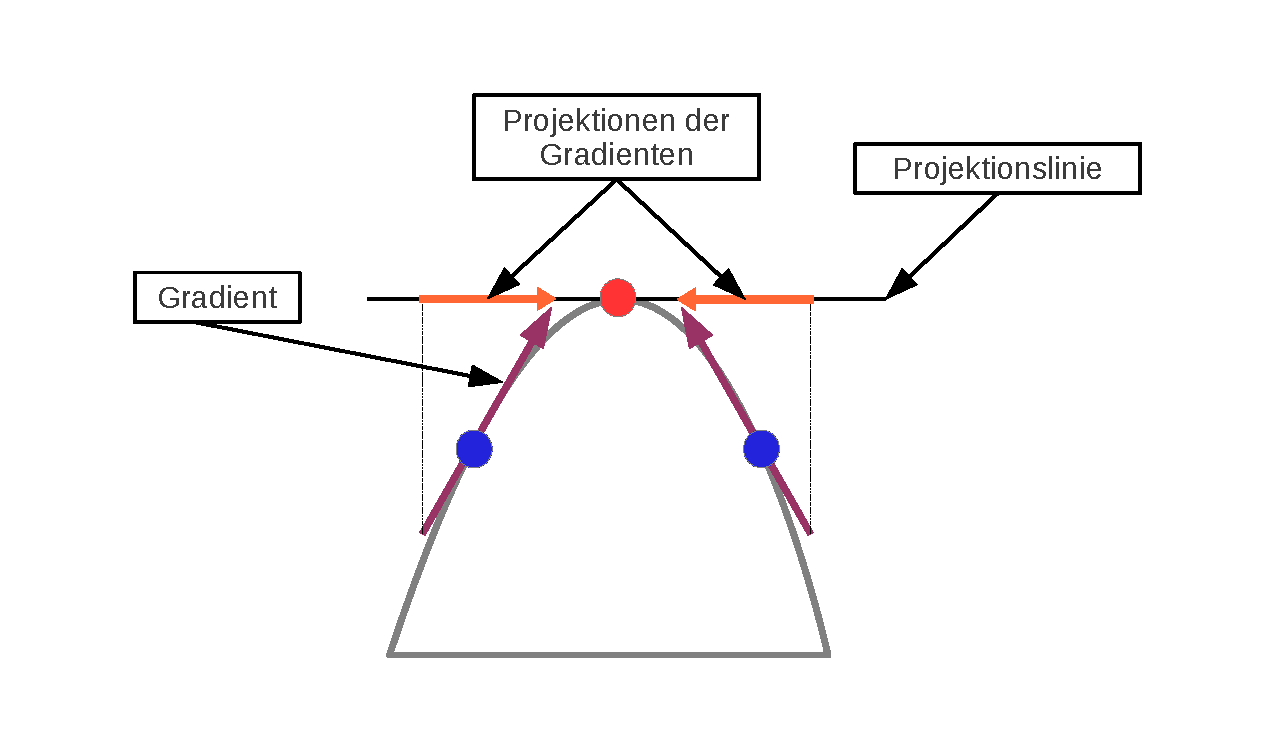
\includegraphics[width=1.0\linewidth]{./fig/paper_ridge_point_detection.pdf}
\caption{Ridge Point Detection. Der rote Punkt ist ein lokales Maximum auf dem Gebirgskamm. Die blauen Punkte liegen sich
gegenüber und umschließen den roten Punkt. Ihre auf die Projektionlinie projizierten Gradientenrichtungen zeigen in entgegengesetzte Richtungen. Der rote Punkt bildet somit eine \emph{sign barrier} für die beiden Richtungen.}
\label{fig:paper_ridge_point_detection}
\end{figure}
\FloatBarrier
\noindent
Die Idee des Algorithmus ist, Projektionslinien durch die Distance Map zu legen und das Verhalten der Gradientenbeträge
auf diesen Lininen zu beobachten. Man stellt fest, dass sich dabei mehrere Muster von Vorzeichenwechsel der
Gradientenbeträge erkennen lassen. Diese Muster können dabei ein Indiz für einen Gebirgspunkt und somit für einen Punkt des Skeletts sein. \\
Dabei stellt sich die Frage, wieviele Richtungen mit diesen Linien untersucht werden sollen. Man kann beobachten, dass es
einen Vorzeichenwechsel in den Gradientenbeträgen gibt, wenn die Projektionslinie den Gebirgskamm schneidet. Dementsprechend 
gibt es keinen Vorzeichenwechsel, wenn die Projektionslinie parallel zum Kamm verläuft. Findet man also in einer Richtung
keinen Gebirgskamm, so muss einer in der orthogonalen Richtung liegen. Deshalb genügt es, zwei zueinander senkrechte Richtungen
zu untersuchen. Dabei wählt man die eine Richtung parallel zur x-Achse und die andere Richtung parallel zur y-Achse des untersuchten Bildes.
\begin{figure}
\centering
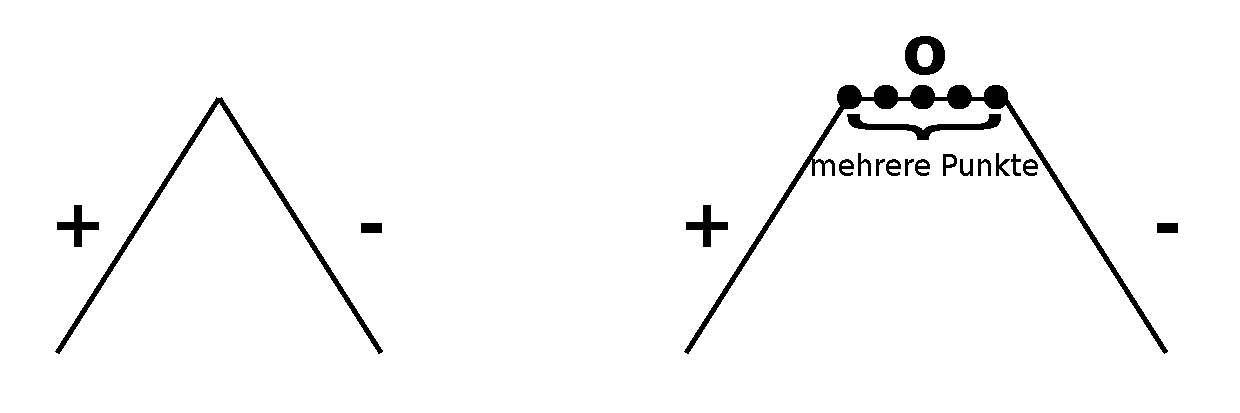
\includegraphics[width=0.8\linewidth]{./fig/muster_strong_good.pdf}
\caption{Muster für Hinweise auf einen Gebirgskamm. Diese beiden Muster sind ein starkes (\emph{strong}, linke Abbildung) und ein gutes (\emph{good}, rechte Abbildung) Indiz für einen Punkt auf dem Gebirgskamm.}
\label{fig:muster_strong_good}
\end{figure}
Es existieren insgesamt vier Muster, die auf einen Gebirgskamm deuten. Zwei davon sind in Abbildung \ref{fig:muster_strong_good}
zu sehen. Die Muster beschreiben, in welcher Weise Vorzeichenwechsel zwischen zwei benachbarten Pixeln auftreten können. Die Symbole $+$ und $-$ die Richtungen der Gradienten. $+$ ist eine positive Richtung (bergauf), $-$ eine negative Richtung (bergab) auf einer Projektionslinie. Das Symbol $\circ$ besagt, dass sich in diesem Bereich der Gradient nicht ändert, da der Grauwert im nächsten Nachbarpunkt gleich ist. Die linke Abbildung entspricht genau der Beobachtung, wie sie anhand Abbildung
\ref{fig:paper_ridge_point_detection} beschrieben wurde. Schneidet die Projektionslinie einen Punkt auf dem Gebirgskamm,
erzeugt dieser Punkt einen Vorzeichenwechsel zwischen den beiden Punkten, die den Punkt auf dem Kamm umschließen. Die rechte
Abbildung zeigt, dass es mehrere Punkte hintereinander in der Distance Map mit dem gleichen Grauwert geben kann, aber auch ein
Hinweis für einen Gebirgskamm sind. Dies entspricht im Grauwertgebirge einem Plateau.\\
Der Algorithmus sucht nun in x -und in y Richtung - von oben nach unten und von links nach rechts - in der Distance Map nach diesen Mustern und markiert die Punkte nach den Eigenschaften \emph{strong}, \emph{good}, \emph{weak} und \emph{none}. 
Diese Markierung gibt die Stärke der Sicherheit des Punktes wieder, ein Punkt auf dem Gebirgskamm zu sein und somit zum Skelett zu gehören. \\
Wurden alle Punkte in beide Richtungen untersucht, hat der Algorithmus zu jedem Punkt das richtige Label gefunden und alle Punkte, die zu einem Gebirgskamm gehören \cite{extracting_skeletons_distancemaps}. Diese Labels werden weiter benutzt, um eine Graphenrepräsentation des Skeletts zu erstellen.
\section{Weitere Verfahren}
\label{sec:weitere_verfahren}
\Autor{Christopher Kroll}\\ \\
Neben Thinning und Distanztransformation bilden Algorithmen, die auf kritische Punkte basieren, die dritte Kategorie. Hier werden kritische, bzw. wichtige Punkte detektiert, die dann zu einem Skelett verbunden werden. Zwei Vertreter dieser Kategorie sind der einfache Kritische-Punkte-Ansatz und die Triangulations-Technik. \\ 
Beim einfachen Kritische-Punkte-Ansatz wird das Quellbild spalten- oder zeilenweise durchgegangen. Werden Objektpixel gefunden, so wird die Mitte dieses 'Objektpixelblocks' markiert. Dies sind die kritischen Punkte, die nach der Markierung verbunden werden und somit das Skelett bilden. Ein Nachteil dieses Ansatzes ist, dass abh"angig von der Lage des Objektes und der Wahl, ob das Quellbild zeilen- oder spaltenweise durchlaufen wird unterschiedliche Ergebnisse erzielt werden, das Verfahren ist somit nicht isotrop. Abbildung \ref{fig:isotrop} zeigt die Skelettierung bei bei zeilenweiser Durchlaufen des Bildes. Abh"angig von der Lage des Objektes ergibt sich ein anderes Skelett. Wenn dieses Objekt spaltenweise durchlaufen werden w"urde, w"urde man beim rechten Kreuz eine horizontale statt vertikale Linie erhalten. Dieses Verfahren ist deswegen daf"ur geeignet, wenn man die Lage des Objektes und das gew"unschte Ergebnis vorher kennt, bzw. die Lage vor der Skelettierung beeinflussen lassen kann.
\begin{figure}
\centering

\includegraphics[width=0.8\linewidth]{./fig/isotrop.png}
\caption{Skelettierung beim einfachen Kritische-Punkte-Ansatz und die Ver"anderung bei der Drehung}
\label{fig:isotrop}
\end{figure}
\\ \\
Zu erw"ahnen ist au"serdem, dass es neben diesen drei vorgestellten Skelettierungskategorien noch weitere Algorithmen gibt, die jedoch sehr speziell und sich dadurch schwer kategorisieren lassen (zum Beispiel das Hamilton-Jacobi-Skelett).
\chapter{Verwandte Arbeiten}
\Autor{Sandra Schröder}\\\\
Zum Thinning und zur Distanztranformation gibt es viele wissenschaftliche Ansätze. 
Im Rahmen einer Literaturrecherche waren zwei Arbeiten besonders interessant, die in den nächsten Abschnitten zusammengefasst werden. 
\section{Extracting Skeletons From Distance Maps}
\Autor{Sandra Schröder}\\\\ 
In dem Paper \emph{Extracting Skeletons from Distance Maps} beschreibt der Autor einen Algorithmus, der effizient und schnell
aus einem distanztransformierten Bild ein Skelett extrahiert \cite{extracting_skeletons_distancemaps}. Der Autor legt besonders hohen Wert darauf, dass die Extraktion keine komplizierten Berechnungen beinhaltet. Er möchte vor allem auf die Berechnung
von Ableitungen höherer Ordnung und die Auswertung von komplexen Gleichungen verzichten. Das Verfahren, welches der Autor zur 
Extraktion der Skelettlinien eines Objekt vorstellt, ist die sogenannte \emph{Ridge Point Detection} (deutsch: \emph{Gebirgskammdetektion}). Dabei nutzt der Autor eine grundlegende Eigenschaft der Distance Map. Wie in Abschnitt \ref{sec:distanztransformation} beschrieben, ist die Distance Map ein Grauwertgebirge, wobei der Gebirgskamm zentriert im Objekt liegt. Betrachtet man nur diesen Teil der Distance Map und projiziert ihn auf das Originalbild, 
lässt sich eine skelett-artige Beschreibung des Objekts erkennen.\\\\
%TODO: Vielleicht ein Bild dazu?
Die Gebirgskammdetektion ist ein gradientenbasiertes Verfahren. Liegt ein Punkt auf den Gebirgskamm, so hat er in 
seiner unmittelbaren Umgebung den größten Abstand zum Objektrand und den größten Grauwert relativ zu seinen Nachbarn. Dieser Punkt ist somit ein lokales Maximum. Aufgrund dieser Tatsache eignet  sich der Gradient am besten, um solch einen Punkt zu detektieren. Der Gradient zeigt nach Definition in die Richtung des stärksten Anstiegs. Dies bedeutet, dass der Gradient eines Punktes, der nicht auf dem Kamm liegt, in die Richtung des Kammes zeigt. Wählt man nun Punkte näher am Kamm, so wird der Anstieg
geringer, da die Differenz zwischen dem Grauwert des betrachteten Gebirgspunktes und dem aktuell gewählten Punkt kleiner wird. Überquert man den Kamm, kehrt sich die Richtung des Gradienten um und zeigt wieder zum Kamm. Hier findet ein Vorzeichenwechsel des Gradientenbetrags statt. Der Punkt auf dem Gebirgskamm bildet eine \emph{sign barrier} zwischen den Gradientenbeträgen der sich gegenüberliegenden Punkte, wobei sich der Gebirgspunkt zwischen diesen beiden Punkten befindet. Diese
Beobachtung ist in Abbildung \ref{fig:paper_ridge_point_detection} dargestellt. Es ist ein Querschnitt eines Grauwertgebirges
abgebildet. Legt man nun eine Projektionslinie genau durch das lokale Maximum (roter Punkt), und projiziert die Gradienten (violette Pfeile) der sich gegenüberliegenden Punkte (blau) auf diese Linie, so kann man erkennen, dass die Projektionen der Gradienten (orangene Pfeile) genau in die entgegengesetzte Richtung zeigen.\
\begin{figure}
\centering
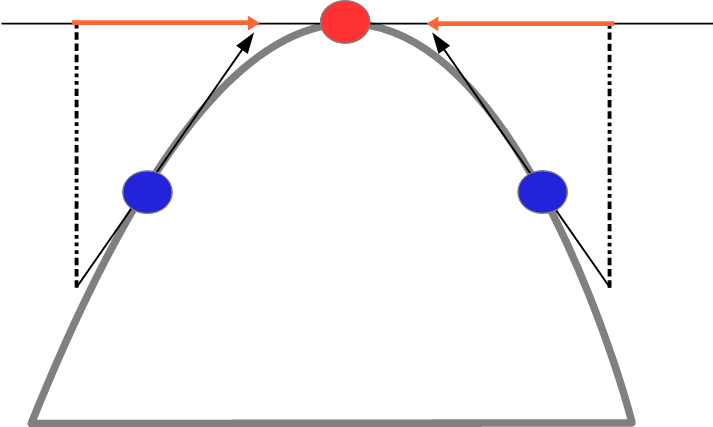
\includegraphics[width=1.0\linewidth]{./fig/paper_ridge_point_detection.png}
\caption{Ridge Point Detection. Der rote Punkt ist ein lokales Maximum auf dem Gebirgskamm. Die blauen Punkte liegen sich
gegenüber und umschließen den roten Punkt. Ihre auf die Projektionlinie projizierten Gradientenrichtungen zeigen in entgegengesetzte Richtungen. Der rote Punkt bildet somit eine \emph{sign barrier} für die beiden Richtungen.}
\label{fig:paper_ridge_point_detection}
\end{figure}
Die Idee des Algorithmus ist, Projektionslinien durch die Distance Map zu legen und das Verhalten der Gradientenbeträge
auf diesen Lininen zu beobachten. Der Autor hat festgestellt, dass sich dabei mehrere Muster von Vorzeichenwechsel der
Gradientenbeträge erkennen lassen. Diese Muster können dabei ein Indiz für einen Gebirgspunkt und somit für einen Punkt des Skeletts sein. \\
Dabei stellt sich die Frage, wieviele Richtungen mit diesen Linien untersucht werden sollen. Man kann beobachten, dass es
einen Vorzeichenwechsel in den Gradientenbeträgen gibt, wenn die Projektionslinie den Gebirgskamm schneidet. Dementsprechend 
gibt es keinen Vorzeichenwechsel, wenn die Projektionslinie parallel zum Kamm verläuft. Findet man also in einer Richtung
keinen Gebirgskamm, so muss einer in der orthogonalen Richtung liegen. Deshalb genügt es, zwei zueinander senkrechte Richtungen
zu untersuchen. Dabei wählt man die eine Richtung parallel zur x-Achse und die andere Richtung parallel zur y-Achse des untersuchten Bildes.
\begin{figure}
\centering

\includegraphics[width=0.8\linewidth]{./fig/muster_strong_good}
\caption{Muster für Hinweise auf einen Gebirgskamm. Diese beiden Muster sind ein starkes (\emph{strong}, linke Abbildung) und ein gutes (\emph{good}, rechte Abbildung) Indiz für einen Punkt auf dem Gebirgskamm. \textbf{TODO die Abbildung ist doof}}
\label{fig:muster_strong_good}
\end{figure}
Es existieren insgesamt vier Muster, die auf einen Gebirgskamm deuten. Zwei davon sind in Abbildung \ref{fig:muster_strong_good}
zu sehen. Die Muster beschreiben, in welcher Weise Vorzeichenwechsel zwischen zwei benachbarten Pixeln auftreten können. Die Symbole $+$ und $-$ die Richtungen der Gradienten. $+$ ist eine positive Richtung (bergauf), $-$ eine negative Richtung (bergab) auf einer Projektionslinie. Das Symbol $\circ$ besagt, dass sich in diesem Bereich der Gradient nicht ändert, da der Grauwert im nächsten Nachbarpunkt gleich ist. Die linke Abbildung entspricht genau der Beobachtung, wie sie anhand Abbildung
\ref{fig:paper_ridge_point_detection} beschrieben wurde. Schneidet die Projektionslinie genau einen Punkt auf dem Gebirgskamm,
erzeugt dieser Punkt einen Vorzeichwechsel zwischen den beiden Punkten, die den Punkt auf dem Kamm umschließen. Die rechte
Abbildung zeigt, dass es mehrere Punkte hintereinander in der Distance Map mit dem gleichen Grauwert geben kann, aber auch ein
Hinweis für einen Gebirgskamm sind. Dies entspricht im Grauwertgebirge einem Plateau.\\
Der Algorithmus sucht nun in x -und in y Richtung - von oben nach unten und von links nach rechts - in der Distance Map nach diesen Mustern und markiert die Punkte nach den Eigenschaften \emph{strong}, \emph{good}, \emph{weak} und \emph{none}. 
%TODO: Doof ausgedrück der folgende Satz
Diese Markierung gibt die Stärke der Sicherheit des Punktes wieder, ein Punkt auf dem Gebirgskamm zu sein. \\
Wurden alle Punkte in beide Richtungen untersucht, hat jeder Punkt ein passendes Label. Diese Labels werden weiter benutzt, um eine Graphenrepräsentation des Skeletts zu erstellen.\\
Der Algorithmus findet zu jedem Punkt das richtige Label und alle Punkte, die zu einem Gebirgskamm gehören \cite{extracting_skeletons_distancemaps}. Abbildung \ref{fig:paper_ergebnis} zeigt ein Ergebnis des Algorithmus. Die gestrichelte Linie in der rechten Abbildung beschreibt das theoretische Skelett, die grau unterlegten Punkte sind die vom Algorithmus gewählten Punkte, die zu einem Gebirgskamm gehören und einem Skelettpunkt entsprechen.
\begin{figure}
\centering
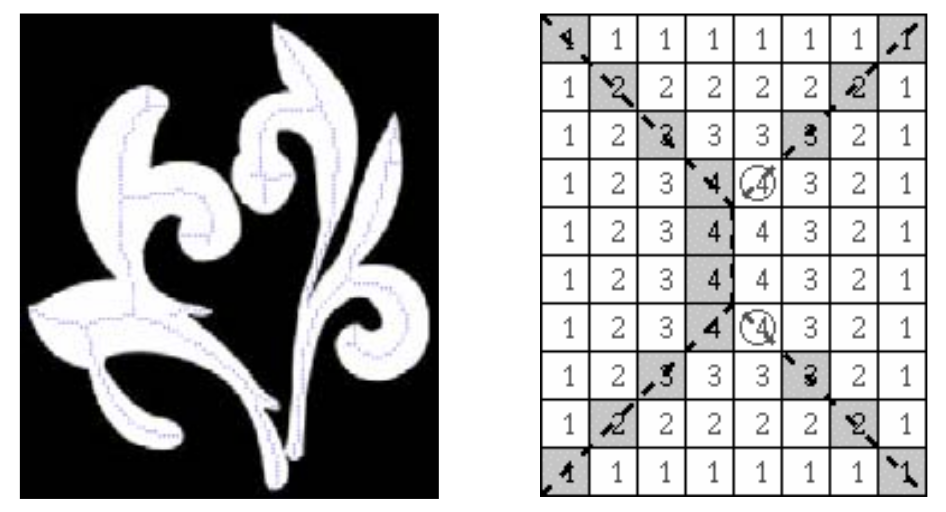
\includegraphics[width=0.7\linewidth]{./fig/paper_ergebnis}
\caption{Ergebnis der Ridge Point Detection \cite{extracting_skeletons_distancemaps}. Links: Graphische Darstellung. Rechts: Darstellung als Bildmatrix. }
\label{fig:paper_ergebnis}
\end{figure}
\newpage
\section{A Fast Parallel Algorithm for Thinning Digital Patterns} 
\Autor{Johannes Böhler}\\\\
Der Algorithmus ist insgesamt in mehrere Iterationen unterteilt. Die Randpixel des Musters werden Schicht für Schicht abgetragen. Die Iterationen sind selbst wiederum in mehrere Subiterationen unterteilt. Das Abtragen der „Schichten“ wird somit in zwei unterschiedliche Phasen aufgespalten
Mit Hilfe der ersten Subiteration werden sowohl Süd- und Ostgrenzpunkte als auch Nordwest Eckpunkte entfernt. \\


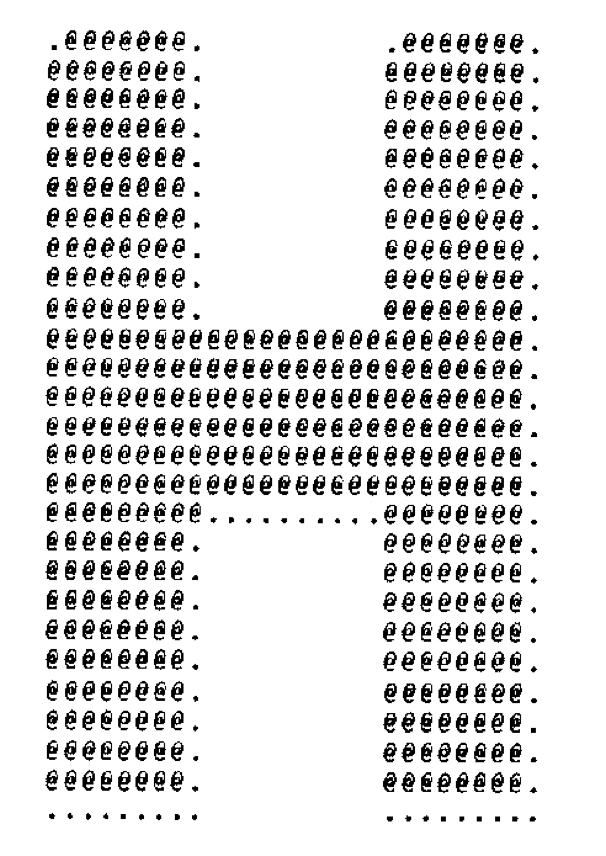
\includegraphics[width=4cm]{Res/SuedOst.png}


Das entfernen von Nord- und Westgrenzpunkten sowie von Südosteckpunkten erfolgt in der zweiten Subiteration.\\

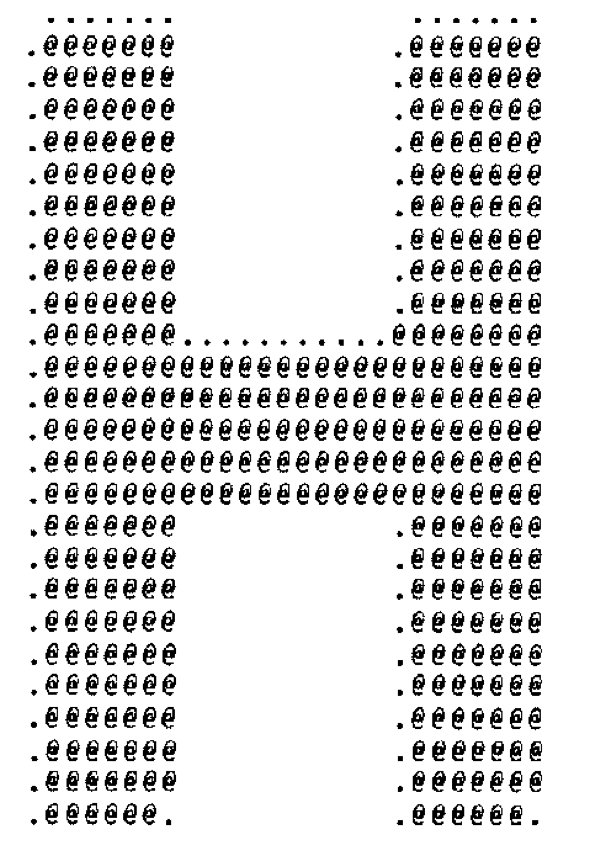
\includegraphics[width=4cm]{Res/NordWest.png}

\subsection{Anforderungen an den Algorithmus}

Das Rauschen, welches der Algorithmus verursacht soll so gering wie möglich gehalten werden.
Das Skelett des Ursprungsmusters soll die Endpunkt- und Pixelverbundenheit erhalten.
Endpunktverbundenheit bedeutet, dass sich zwischen zwei Endpunkten eines Skeletts keine unverbundenen Stellen befinden.
Das Skelett soll nach Durchlaufen des kompletten Algorithmus in einheitlicher Dicke von einem Pixel vorliegen.
Der Algorithmus soll möglichst schnell und effizient arbeiten um Echtzeitfähigkeit gewährleisten zu können.\\


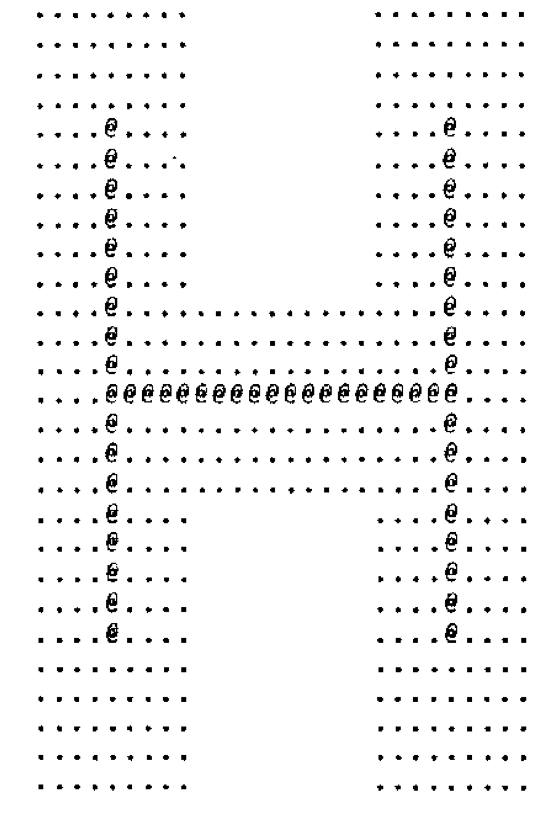
\includegraphics[width=4cm]{Res/Skelett.png}

\subsection{Ablauf des Algorithmus}

Es wird davon ausgegangen zu Beginn ein binär digitalisiertes Bild vorliegen zu haben.
Die Pixel werden mit Hilfe einer zweidimensionalen Matrix IT durchlaufen, deren Wert an der jeweiligen Stelle IT(i,j) entweder 0 oder 1 ist.
Mit Muster ist die Menge an Pixeln gemeint, welche den Wert eins haben.
Es werden nun in Abhängigkeit von den 8 Nachbarpixeln, Punkt für Punkt iterative Transformationen auf die Matrix angewendet.

Der neue Wert eines Pixels während der n-ten Iteration hängt von dem eigenen Wert während der (n-1)ten Iteration und den Werten der acht Nachbarn während der (n-1)ten Iteration ab. Dies ermöglicht paralleles Transformieren mehrerer Bildpunkte. 
Die Bedingungen, welche zum Ausführen der Transformation erfüllt sein müssen werden über ein 3x3 Pixel Fenster abgefragt. Der Punkt P1 über dessen Transformation entschieden wird, ist mit allen acht Nachbarn verbunden.\\

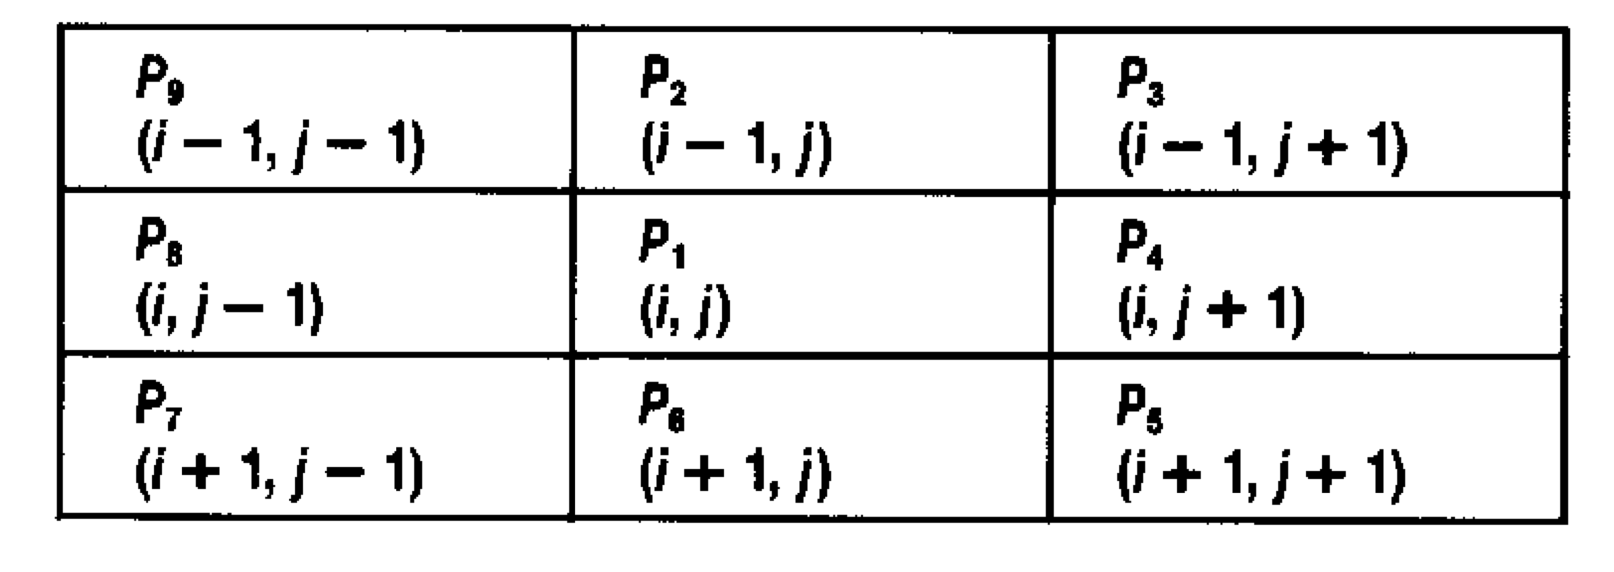
\includegraphics[width=8cm]{Res/PixelNachbarschaft.png}


Der Algorithmus entfernt alle Randpunkte des Musters, außer den Pixeln welche Bestandteil des Skeletts sind. Um die Verbundenheit des Skeletts zu gewährleisten wird ein  Iterationsschritt in zwei Subiterationen aufgeteilt.

In der ersten Subiteration wird der Punkt P1 aus dem Muster gelöscht wenn er folgende Bedingungen erfüllt:\\ \\
a)2<=B(P1)<=6     
Bà Anzahl der Nachbarn von P1 !=0
Die Anzahl der Nachbarn von P1 welche den Wert 1 haben, muss somit zwischen 2 und 6 liegen.\\ \\
b) A(P1)=1
AàAnzahl der „01“-Folgen 
Die Anzahl der 01 Folgen in der geordneten Folge P2,P3...P9 muss genau eins betragen.\\ \\
c) P2*P4*P6=0  
Mindestens ein Pixel der Pixelmenge P2, P4, P6 muss den Wert Null haben.\\ \\
d) P4*P6*P8=0
Mindestens ein Pixel der Pixelmenge P4, P6, P8 muss den Wert Null haben.
\\

Sind alle Bedingungen a, b ,c und d erfüllt so wird der Wert des Pixels auf 0 gesetzt.
Dies bedeutet dass er kein Teil des Skelett-Musters mehr ist.
Wird eine der Bedingungen nicht erfüllt, so bleibt der Pixelwert bei 1.\\

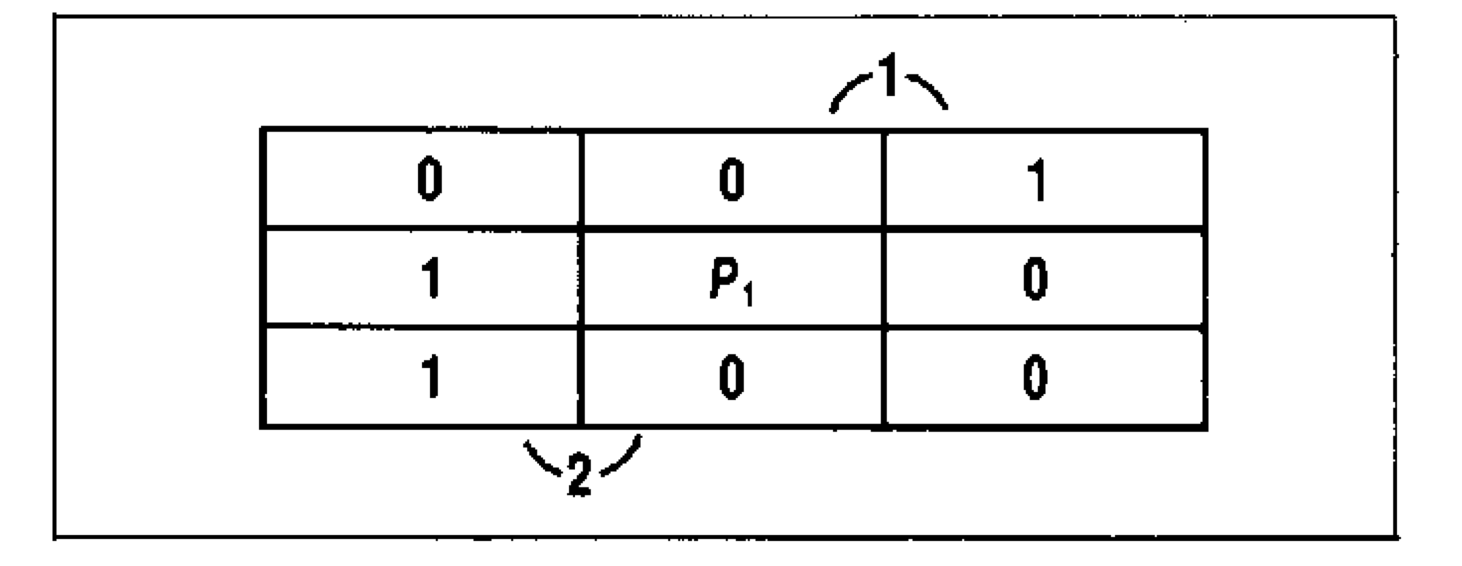
\includegraphics[width=8cm]{Res/01Folgen.png}


In der zweiten Subiteration wird P1 gelöscht falls folgende Bedingungen gelten: \\ \\
a) 2<=B(P1)<=6 \\ \\
b) A(P1)=1 \\ \\
c) P2*P4*P8=0 \\ \\
d) P2*P6*P8=0 \\ \\
In der zweiten Subiteration haben sich nur die Bedingungen c und d geändert.\\

Um die Bedingungen der ersten Subiteration zu erfüllen muss
P4=0 oder P6=0 oder (P2=0 und P8=0)  erfüllt sein.
Dies impliziert dass P1 entweder Süd- oder Ost-Grenzpunkt, oder Nordwesteckpunkt ist.
Um die Bedingungen der zweiten Subiteration zu erfüllen muss
P2=0 oder P8=0 oder (P4=0 und P6=0) sein.
Das heißt P1 ist Nord -oder West-Grenzpunkt oder Südosteckpunkt ist.

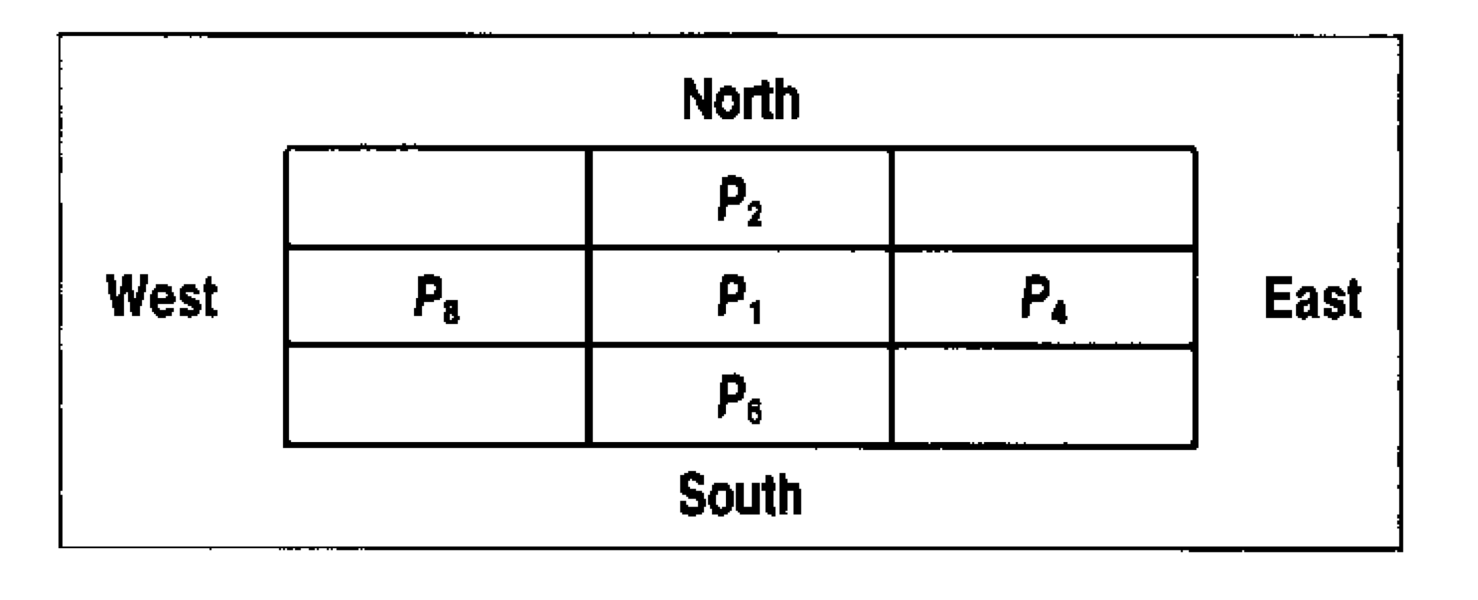
\includegraphics[width=8cm]{Res/Orientierung.png}


Während mit Bedingung a (2<=B(P1)<=6) die Endpunkte des Skeletts erhalten werden, so wird mit Bedingung b (A(P1)=1) die Auslöschung von Punkten zwischen den Endpunkten der Skelettlinie verhindert.\\

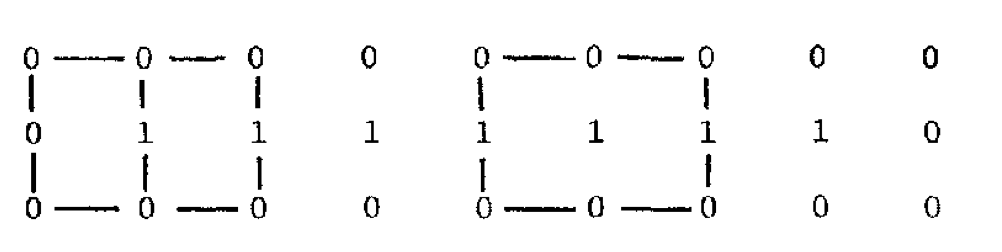
\includegraphics[width=8cm]{Res/EndpktVerbheit.png}

In der Matrix Search M befinden sich während der ersten Iteration alle Pixel die gelöscht werden dürfen, da sie den Bedingungen der ersten Iteration genügen. Ist dies nicht der Fall, so ist der Counter=0 und der Algorithmus beendet, da es anscheinend keine zu löschenden Pixel mehr gibt. Die Skelettierung ist somit beendet.
Falls der Counter ungleich null ist, werden die Pixel welche den Bedingungen genügen von der Matrix IT (Skelett-Muster) abgezogen, der Counter wird null gesetzt und es wird zur zweiten Iteration fortgeschritten. Dort findet der Ablauf mit veränderten Bedinungen c und d nochmals statt. Ist auch nach dem Durchlaufen der zweiten Subitertation der Counter ungleich null so wird der Vorgang iterativ fortgeführt.\\




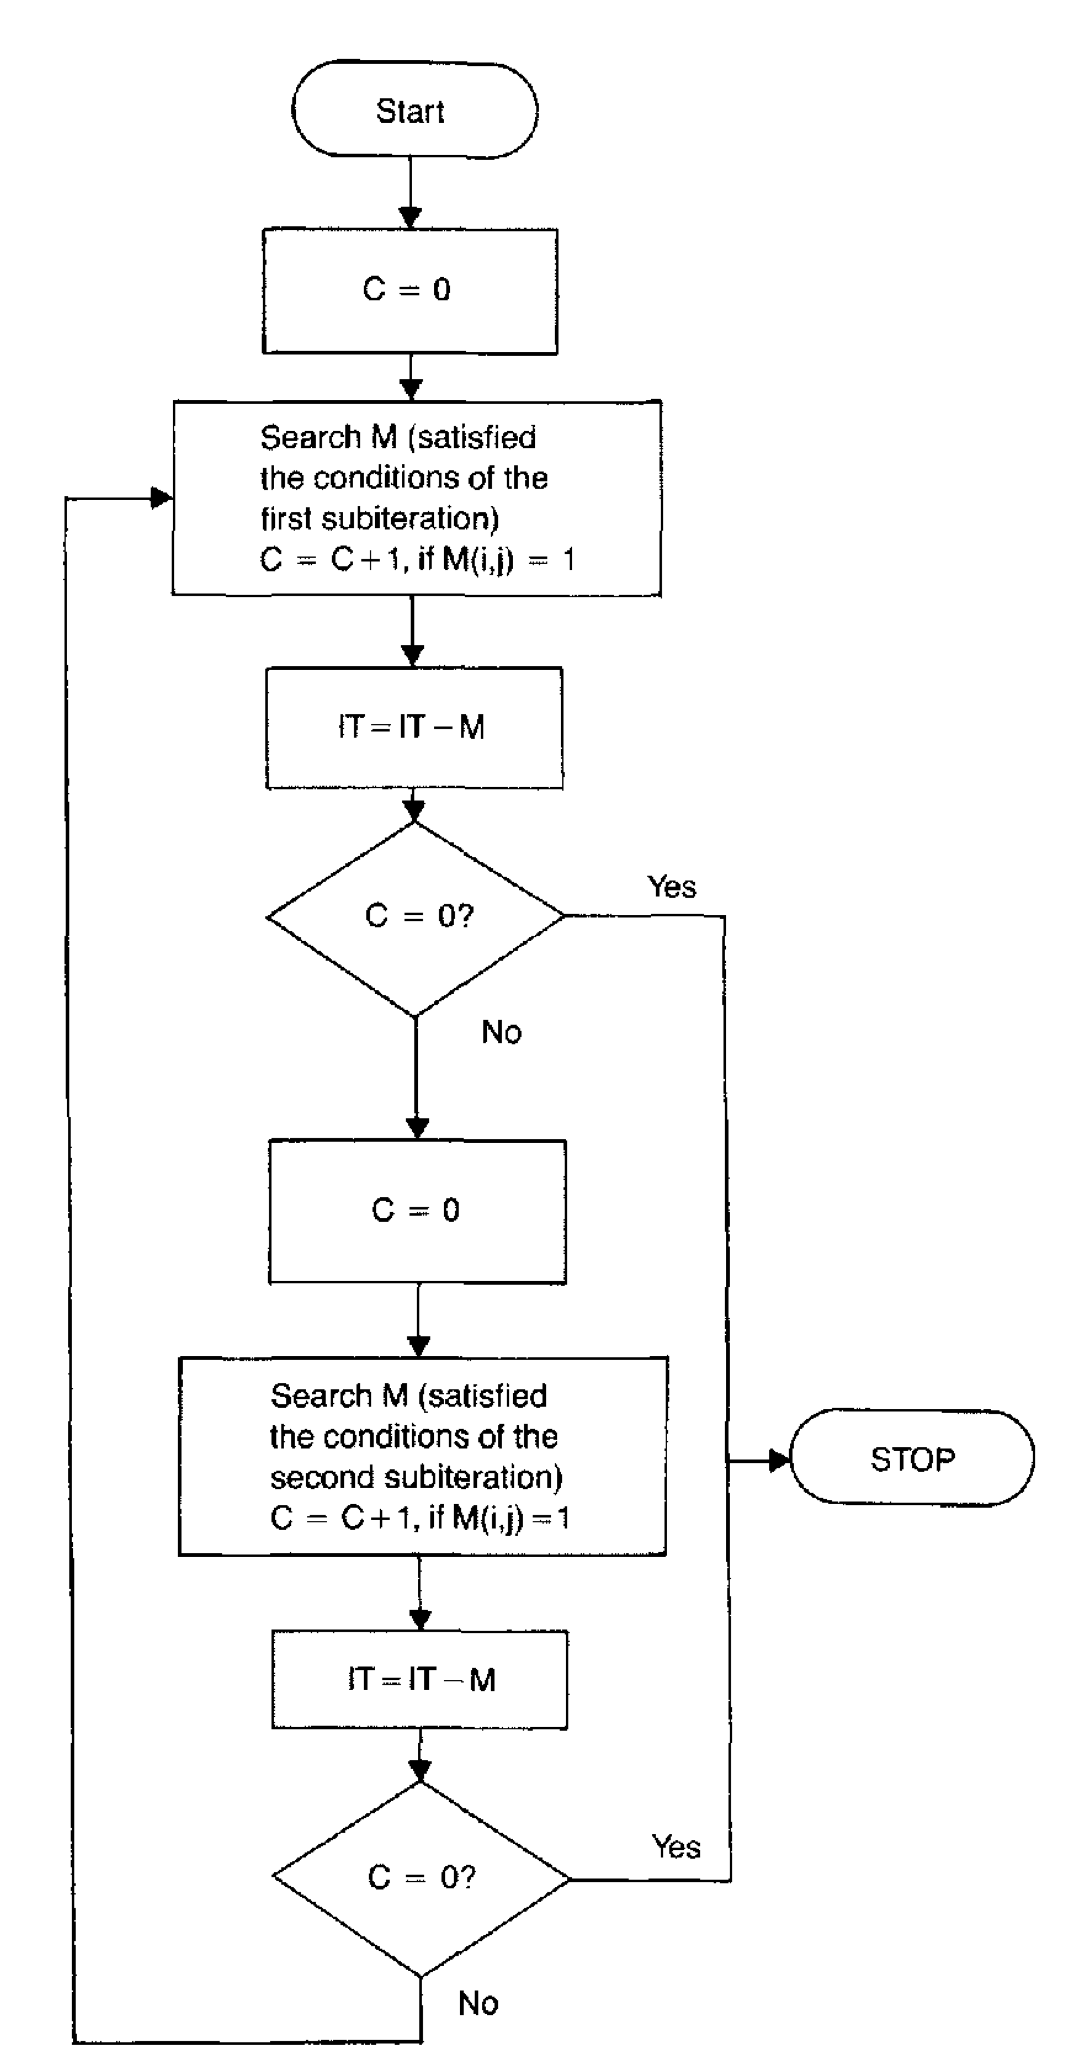
\includegraphics[width=6cm]{Res/AlgUebersicht.png}


Der Algorithmus erzielt sehr gute Ergebnisse im Bezug auf Verbundenheit, und Rauschsicherheit bei Randpunkten. Die Bedingungen welche zum Auffinden der zu löschenden Randpunkte führen sind sehr simpel. Durch den Bezug auf die n-1te Iteration zur Abfrage der Bedingungen kann der Algorithmus sehr schnell ausgeführt werden, da keine Warteabhängikeiten bestehen.

\chapter{Implementierung der Algorithmen}
\Autor{Sandra Schröder}\\\\
Im Rahmen des Projekts wurden zwei Algorithmen für die Skelettierung implementiert. Dies ist zum einen
die Skelettierung nach Thinning nach dem Algorithmus der in Abschnitt \ref{subsec:fastparallel} beschrieben wurde. Die Skelettierung mittels Distanztransformation wurde nach einer eigenen Idee entwickelt und
umgesetzt.\\
Die Skelettierung läuft in zwei Schritten ab. Erst wird der Spieler segmentiert. Man erhält als
Ergebnis ein Binärbild, welches im zweiten Schritt weiterverarbeitet wird, um ein Skelett zu extrahieren. 
Die Segmentierung des Spielers ist bei beiden Ansätzen identisch.
In diesem Kapitel wird die Umsetzung der Algorithmen anhand signifikanten Codeausschnitten der Implementierungen vorgestellt. Ein Überblick über die technische Umsetzung gibt einen Eindruck über die
verwendeten Programmiersprachen und Arbeitsumgebungen.
\section{Technische Umsetzung}
\Autor{Christopher Kroll}\\
F"ur die Implementierung wurden die bereitgestellten iMacs am Informatikum in Stellingen gew"ahlt. Der Vorteil war neben der Performanz die schon eingerichtete Arbeitsumgebung.\\
Um die Verbindung zu der Kinect herzustellen, wurde das quelloffene Framework libfreenect  der OpenKinect-Gruppe benutzt. Libfreenect bietet Treiber und Bibliotheken, um zum Beispiel die Bilder der Kamera anzuzeigen oder den eingebauten Motor zu steuern. \\
Um die empfangenen Bilder verarbeiteten zu k"onnen wurde die Bibliothek OpenCV eingesetzt. Sie unterst"utzt unter anderem beim Speichern und Laden von Bildern und bei der Segmentierung. \\
Der Gro"steil der Programmiierung erfolgte in der Sprache Python. Hierbei handelt es sich um eine leicht zu erlernende Skriptsprache. Allerdings traten im Laufe des Projektes Performanzprobleme bei der Implementierung des Thinning-Algorithmus auf. Aus diesem Grund wurde "uber einen Python-Wrapper der in C++ implementierte Algorithmus eingebaut. N"aheres dazu wird in Kapitel \ref{implThinning} beschrieben.
Als Entwicklungsumgebung wurde spyder f"ur die Python-Programmierung und Xcode f"ur die C++-Programmierung benutzt.
TODO numpy
\section{Spieler-Segmentierung}
\Autor{Sandra Schröder}\\\\
Es wird anhand der Tiefeninformation segmentiert, die die Kinect liefert. Der Open-Source-Treiber für die Kinect - \emph{Freenect} - bietet Funktionen für den Zugriff auf die
Tiefenwerte. Die Funktion \texttt{pretty\_depth} des Moduls
\texttt{frame\_convert} normiert die Tiefenwerte auf das 
Intervall $[0,...,255]$. 
\lstset{
caption={Tiefenwerte zurückgeben}
\label{lst:getdepth}
}
\lstinputlisting{./listing/getdepth.py}
Um nicht für jeden einzelnen Pixel die Bedingung zu überprüfen, ob er den Schwellwert für die Segmentierung überschreitet beziehungsweise unterschreitet, wird die effiziente Numpy-Funktion \texttt{logical\_and} benutzt, die global auf dem Bild arbeitet und für das gesamte Bild die Schwellwertbedingung prüft. Eine pixelweise Überprüfung wäre mit Python eine ineffiziente Lösung.\\ Für den Schwellwert werden zwei 
Werte definiert, um ein Intervall festzulegen, in dem sich das Objekt befinden darf. In Listing \ref{lst:spielersegmentierung} legen die Variablen \texttt{current\_depth} und \texttt{threshold} das Intervall fest. 
\lstset{
caption={Spielersegmentierung in Python}
\label{lst:spielersegmentierung}
}
\lstinputlisting{./listing/player_segmentation.py}
Da die Funktion auf Numpy-Arrays arbeitet, muss das Bildobjekt zuvor in ein Array umgewandelt werden. 
Es wurden vorgefertigte Funktionen von OpenCV benutzt, die diese Konvertierung vornehmen. 
\section{Skelettierung mittels Thinning} 
\label{implThinning}
\Autor{Christopher Kroll}
Da man sich schon durch den Seminarteil mit dem Algorithmus 'A Fast Parallel Algorithm for Thinning Digital Patterns' besch"aftigte, fiel die Wahl des Thinning-Algorithmus zun"achst auf diesen.

\section{Skelettierung mittels Distanztransformation}
%Sandra
\Autor{Sandra Schröder}\\\\
Der theoretische Ablauf der Skelettierung wurde bereits im Kapitel \ref{ch:Skelettierung} beschrieben. Zur
Rekapitulation werden die Schritte kurz aufgezählt. \\
Die Skelettierung anhand der Distanztransformation läuft folgendermaßen ab:
\begin{itemize}
\item Bestimmen der Distanztransformation des Binärbildes
\item Berechne den Gradientenbetrag auf der Distance Map
\item Differenz zwischen dem Gradientenbild und der Distance Map bilden
\end{itemize}
Die Distance Map kann mit einer Funktion aus der Bildverarbeitungsbibliothek \emph{OpenCV} einfach berechnet
werden. Die Funktion (Listing \ref{lst:disttransform}) erwartet als Eingabe das Originalbild (\texttt{img}) und ein Bild (\texttt{dist\_img}), um
das Ergebnis speichern zu können (gleiche Größe und Dimension wie das Originalbild). Eine weitere Möglichkeit, die die Funktion bietet, ist die Angabe einer Metrik, nach der der Abstand eines Pixels zum
Hintergrund bestimmt wird. Es wurde die euklidische Metrik benutzt.
\lstset{
caption={Berechnen der Distance Map des Spielers.}
\label{lst:disttransform}
}
\lstinputlisting{./listing/distancetransform.py}
Zur Bestimmung des Gradientenbetrages der Distance Map wurde die Numpy-Funktion \texttt{gaussian\_gradient\_magnitude} genutzt. Die Funktion berechnet den Gradientenbetrag mit Ableitungen
der Gaussfunktion. Die Variable \texttt{sigma} ist die Standardabweichung 
des Gaussfilters. Das Ergebnis dieser Funktion wird in ein Bildobjekt
konvertiert und entsprechend festgelegter Schwellwerte (\texttt{lowerbound}, \texttt{upperbound}) segmentiert.
\lstset{
caption={Gradientenbetrag der Distance Map und Segmentierung des Gradientenbetragsbildes.}
\label{lst:gradient}
}
\lstinputlisting{./listing/gradient.py}
Zur Differenzbildung und endgültigen Berechnung des Distanzskelettes werden die Bildobjekte in Arrays umgewandelt. 
Diese Arrays können einfach voneinander abgezogen werden. 
\lstset{
caption={Differenz zwischen Distance Map und segmentiertem Gradientenbetrag}
\label{lst:difference}
}
\lstinputlisting{./listing/difference.py}
Bei der Implementierung wurden in keinem Fall Operationen ausgeführt, die auf einzelne Pixel zugreifen. Situationen, in denen
pixelweise Operationen durchgeführt werden könnten, wurden
umgangen, indem Arrayoperationen oder Funktionen aus der
OpenCV-Bibliothek benutzt wurden. Ein pixelweiser Zugriff
könnte bei einer Interpretersprache wie Python zu einer sehr langsamen
Ausführung der Skelettberechnung führen.
\chapter{Ergebnisse}
%Sandra
\Autor{Sandra Schröder}
\begin{itemize}
	\item Vergleich der Algorithmen
	\item Anhand der Kriterien: QUELLE!!!
	\begin{itemize}
		\item Erhaltung der Topologie
		\item Pixelkonnektivität
		\item Zentriert
		\item 1 Pixel breit
		\item Robustheit
	\end{itemize}
	\item Vergleich anhand von Screenshots
	\item Echtzeitfähigkeit -> Messungen machen -> Vergleich
	\item Verbesserung des Skeletts (Distanztransformation) mit Breitensuche um Pixelkonnektivität zu erreichen -> Weitere Verbesserungen? -> Ohne Features sondern anhand der weißen Pixel
	\item Anwendung: Vergleich von Posen -> Features bestimmen. Vllt sowas wie "Spannweite" der Pose in x und in y Richtung (Abstand des "linkesten" zum "rechtesten" Pixel). 
\end{itemize}
\section{Vergleich der Algorithmen}
\section{Echtzeitfähigkeit}
\section{Verbesserung der Skelettqualität}
Verbesserung des Skeletts (Distanztransformation) mit Breitensuche um Pixelkonnektivität zu erreichen -> Weitere Verbesserungen? -> Ohne Features sondern anhand der weißen Pixel
%\section{Vergleich von Posen}
%Anwendung: Vergleich von Posen -> Features bestimmen. Vllt sowas wie "Spannweite" der Pose in x und in y Richtung (Abstand des "linkesten" zum "rechtesten" %Pixel). 
\chapter{Zusammenfassung und Ausblick}
\label{ch:ausblick}
\Autor{Christopher Kroll}\\\\
F"ur alle Teammitglieder war das Arbeiten mit Python und der Kinect Neuland. In der Anfangsphase des Projektes musste sich zun"achst in die Programmiersprache und die Funktionsweise der Kamera eingearbeitet werden. Welche Daten die Kinect auf welche Weise liefert und wie diese mit den Frameworks aufgenommen und benutzt werden k"onnen, musste untersucht werden.\\\\
Damit nicht das komplette Blickfeld der Kamera, sondern nur das relevante Objekt, also der Mensch vor der Kamera, skelettiert wird, musste dieser segmentiert werden.\\Aufbauend auf diesem Ergebnis konnte sich mit der Skelettierung und den unterschiedlichen Verfahren gek"ummert werden. In dieser Phase wurde das Ziel der Projektarbeit angepasst. Wurde zun"achst angepeilt ein Bewegungsanalyseprogramm zu schreiben, wurde nun die Konzentration auf eben diese Verfahren gelegt und das Vorhaben war es jetzt Skelettierungsalgorithmen zu implementieren und zu vergleichen.\\\\Die Entscheidung fiel auf eine Skelettierung mittels Distanztransformation und ein Thinning-Verfahren. W"ahrend bei der Distanztransformation ein eigener Ansatz gew"ahlt wurde, entschied man sich durch die Papervorstellung im Seminar einen bereits etablierten Algorithmus f"ur das Thinning zu w"ahlen. Trotz einigen Schwierigkeiten, wie dem Laufzeitproblem in Python und dem Wechsel des Algorithmus, konnten am Ende gute Ergebnisse erzielt und die beiden Verfahren miteinander verglichen werden. \\\\
Es stellte sich heraus, dass das Thinning zwar ein gutes Skelett liefert, aber durch den iterativen Prozess zu langsam ist. Der Wechsel der Programmiersprache brachte zwar einen Leistungszuwachs, dieser war jedoch noch immer zu unbefriedigend bei Anwendung auf Bewegtbilder. F"ur statische Bilder ist dieser Ansatz jedoch geeignet. \\ Die Distanztransformation ist dagegen echtzeitf"ahig. Allerdings liefert dieser Ansatz nicht so ein gutes Skelett wie das Thinning. So ist die Pixelkonnektivit"at nicht gegeben. 
\\
Der Vergleich der Algorithmen hat gezeigt, dass sich abhängig vom Algorithmus die Skelettqualität unterscheidet. Auch die 
Laufzeit ist ein wichtiges Unterscheidungsmerkmal. Vor allem im Hinblick auf die Anforderung Echtzeitfähigkeit.\\\\
Die Skelette, die mit den beiden Algorithmen bestimmt wurden, eignen sich beide für weitere Anwendungen. Allerdings muss bei beiden Algorithmen optimiert werden. Beim Thinning-Algorithmus ist dies die Laufzeit, bei der Skelettierung mittels Distanztransformation ist dies die Skelettqualität. Die Verbesserungen des Distanzskeletts sind vielversprechend. Der nächste Schritt wäre die Integration in die Kinect-Umgebung. Es muss
getestet werden, wie performant dies ist. \\\\ Ist die Skelettierung optimiert, kann man das Ergebnis nutzen, um Anwendungen, wie zum Beispiel die erw"ahnte und zun"achst vorgesehene Bewegungsanalyse zu erstellen.
\chapter{Fazit und Ausblick}
\section{Fazit}
\section{Ausblick}


\bibliographystyle{alpha}
\bibliography{literatur}

\appendix       %Beginn des Anhangs
\chapter{Quellcode}
\label{anhang:quellcode}
\section{Verbesserung der Skelettqualität}
 \lstinputlisting
    [caption={Breitensuche}
       \label{lst:javaclass},
       captionpos=t,language=python]
 {/home/sandra/projects/bildverarbeitung/src/skeleton_improvement.py}

\end{document}
